\section{Plan de implantación}
\par En esta sección se describirá el método de implantación del portal LifeRay 7 en un entorno de producción, de forma que sea integrable con otras instancias de LifeRay.

\subsection{Instalación del Software}
\par Antes de configurar el portal, será necesario instalarlo en el caso de que éste no se encuentre en el sistema. Para instalarlo, se utilizarán los siguientes componentes de software:
\begin{itemize}[-]
    \item LifeRay 7 con Tomcat 8: Web de Descarga
    \item Linux (recomendable que sea una distribución RHEL): Web de Descarga
    \item Oracle Java 8 JDK: Web de Descarga
\end{itemize}
\par Debido al carácter del documento, no se cubrirá cómo instalar el sistema operativo.

\subsection{Instalación de Java 8 JDK}
\par Desde la web de descarga, se deberá descargar el archivo RPM en el caso de utilizar una distribución RHEL o el archivo comprimido en el caso contrario. Para que la guía de implantación sea aplicable a cualquier distribución, se utilizará el archivo comprimido.
Primero se deberá extraer (recomendable extraerlo en \textit{/opt/ o en /usr/share}):

\begin{listing}[style=consola, numbers=none]
> tar xvf jdk.tar.gz
\end{listing}

\par A continuación, se añadirán las variables de entorno:
\begin{listing}[style=consola, numbers=none]
> export JAVA_HOME='/opt/jdk'
> export PATH=$JAVA_HOME/bin:$PATH
\end{listing}

\subsection{Instalación de LifeRay 7}
\par Una vez descargado el archivo, se deberá descomprimir (recomendable en /opt):
\begin{listing}[style=consola, numbers=none]
unzip liferay-ce-portal-tomcat-7.0-ga5-20171018150113838.zip
\end{listing}
\par Con esto, LifeRay quedaría instalado y sólo quedaría configurarlo.


\subsection{Configuración del portal}

\par A continuación se describe cómo configurar el portal para que se pueda realizar la integración. Antes de poder configurar el portal, éste se deberá arrancar como root a menos que se hayan configurado los permisos de otra forma:
\begin{listing}[style=consola, numbers=none]
/opt/liferay-ce-portal-7.0-ga5/tomcat-8.0.32/bin/catalina.sh run
\end{listing}


\subsubsection{Configuración básica}
\par Primero se deberá configurar el nombre y el administrador, tal y como puede verse en la imagen \ref{img:lr1}.

\begin{figure}[H]
\begin{center}
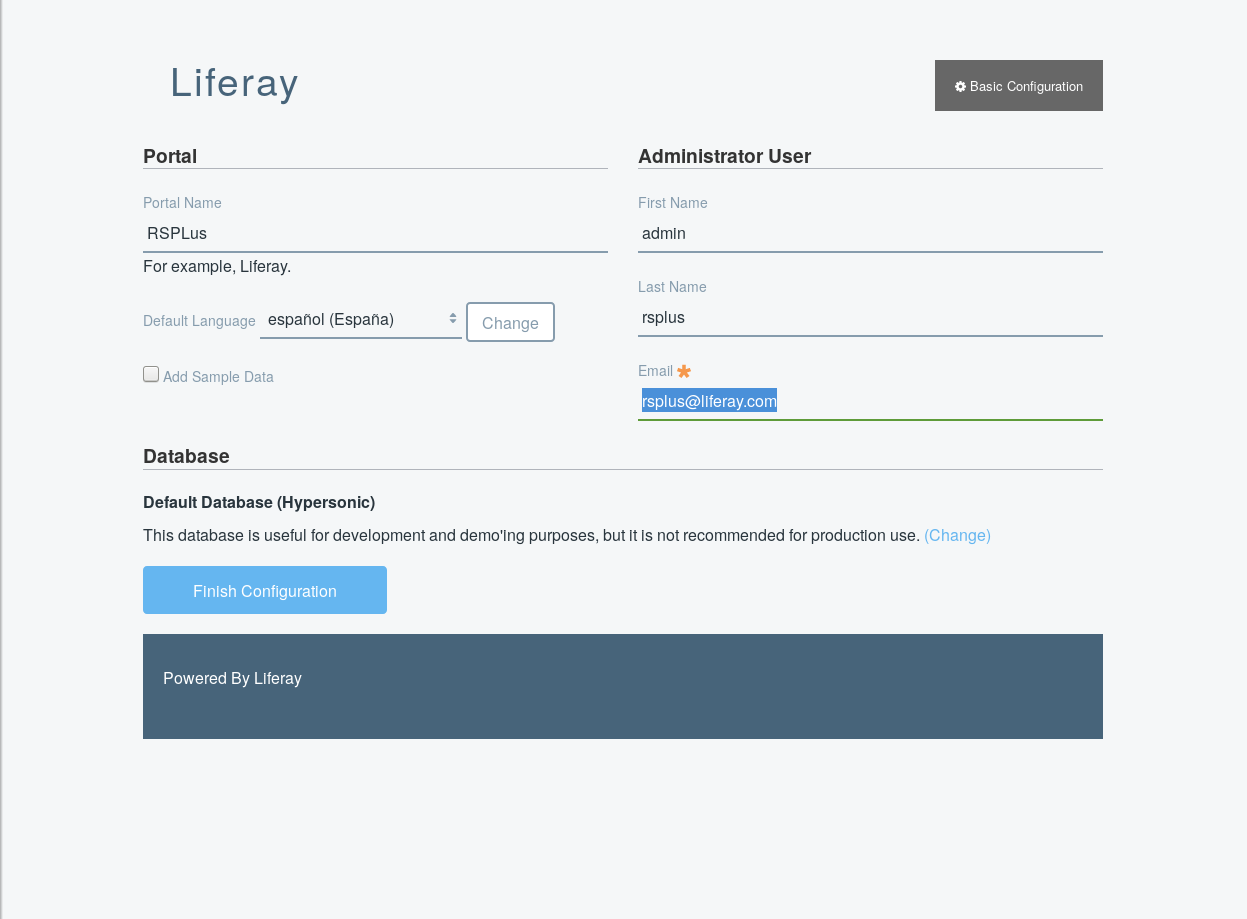
\includegraphics[width=0.8\textwidth]{./img/liferay/1.png}
\end{center}
\caption{Configuración del nombre y del administrador}
\label{img:lr1}
\end{figure}

\par Una vez realizado, pulsar \textit{Finish Configuration} y aceptar las condiciones de uso, así como introducir una contraseña y pregunta de seguridad.

\subsubsection{Configuración de la página base y las subpáginas}
\par Primero se deberá añadir una nueva página pública, tal y como se ve en la imagen \ref{img:lr2}. A continuación, se realiza la configuración inicial (véase la imagen \ref{img:lr3}). Después, se elimina la página inicial tal y como se puede ver en la imagen \ref{img:lr4}. Se procede a crear las subpáginas para \textit{Venta y alquiler} con la opción de añadir la subpágina (véase figura \ref{img:lr5}). Por otro lado, se debe crear una carpeta en Contenidos Web llamada \textit{ComercialesOtrosActivos}, tal y como se puede ver en la imagen \ref{img:lr6}. Tras ello, se debe creae una estructura llamada \textit{OtrosActivos}, como se describe en las imágenes \ref{img:lr7}, \ref{img:lr8}, \ref{img:lr9}.

\begin{figure}[H]
\begin{center}
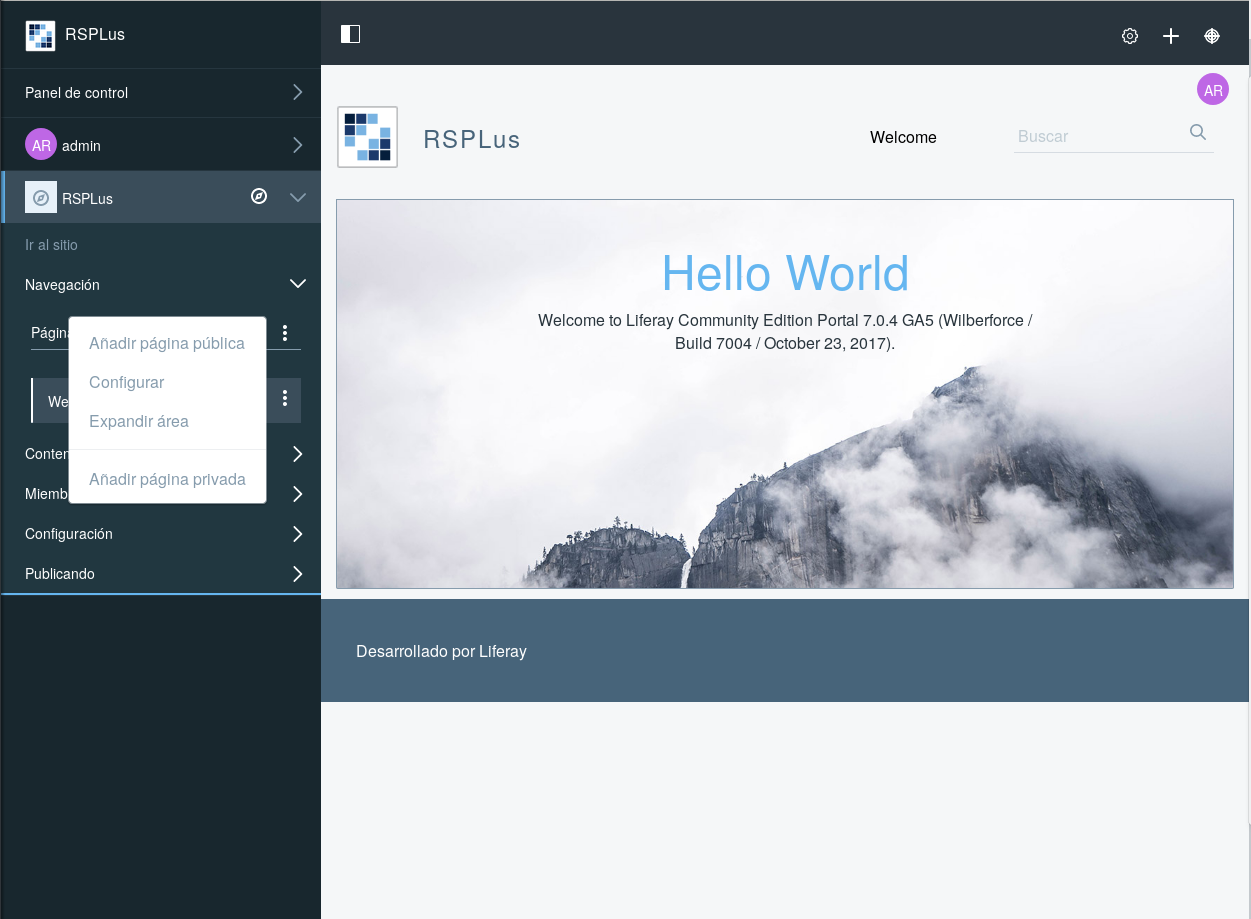
\includegraphics[width=0.8\textwidth]{./img/liferay/2.png}
\end{center}
\caption{Creción de la página base pública}
\label{img:lr2}
\end{figure}

\begin{figure}[H]
\begin{center}
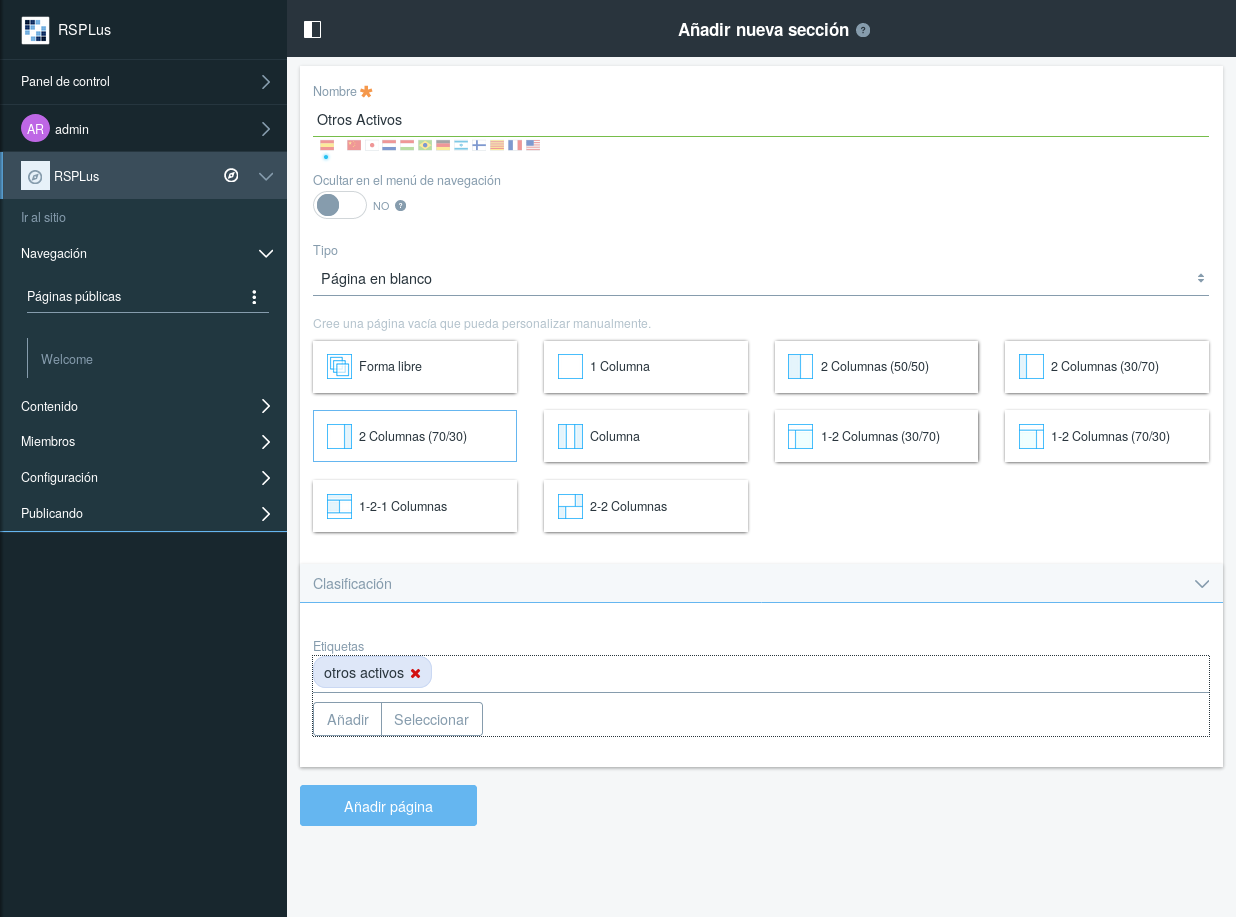
\includegraphics[width=0.8\textwidth]{./img/liferay/3.png}
\end{center}
\caption{Configuración de la página base}
\label{img:lr3}
\end{figure}

\begin{figure}[H]
\begin{center}
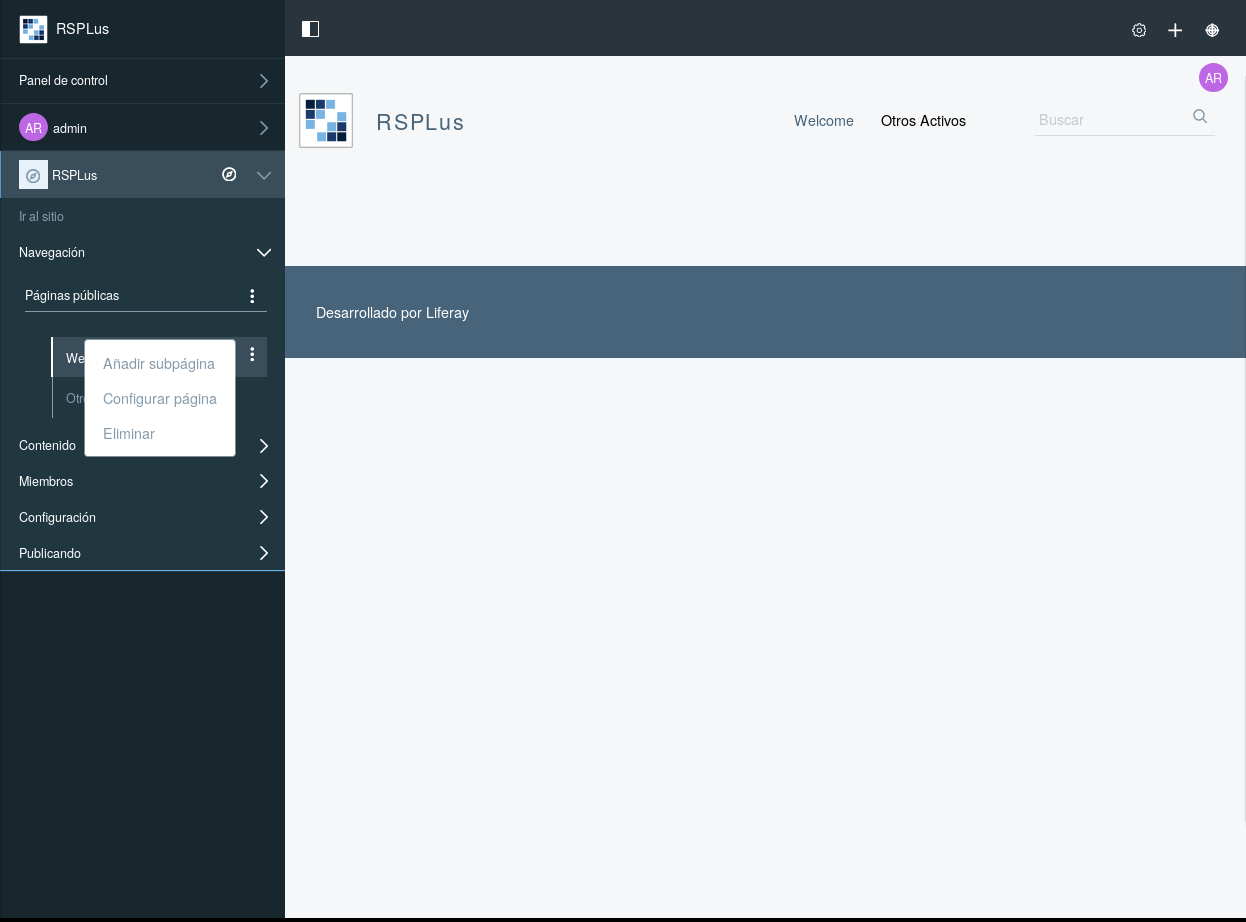
\includegraphics[width=0.8\textwidth]{./img/liferay/4.png}
\end{center}
\caption{Eliminación de la página inicial}
\label{img:lr4}
\end{figure}

\begin{figure}[H]
\begin{center}
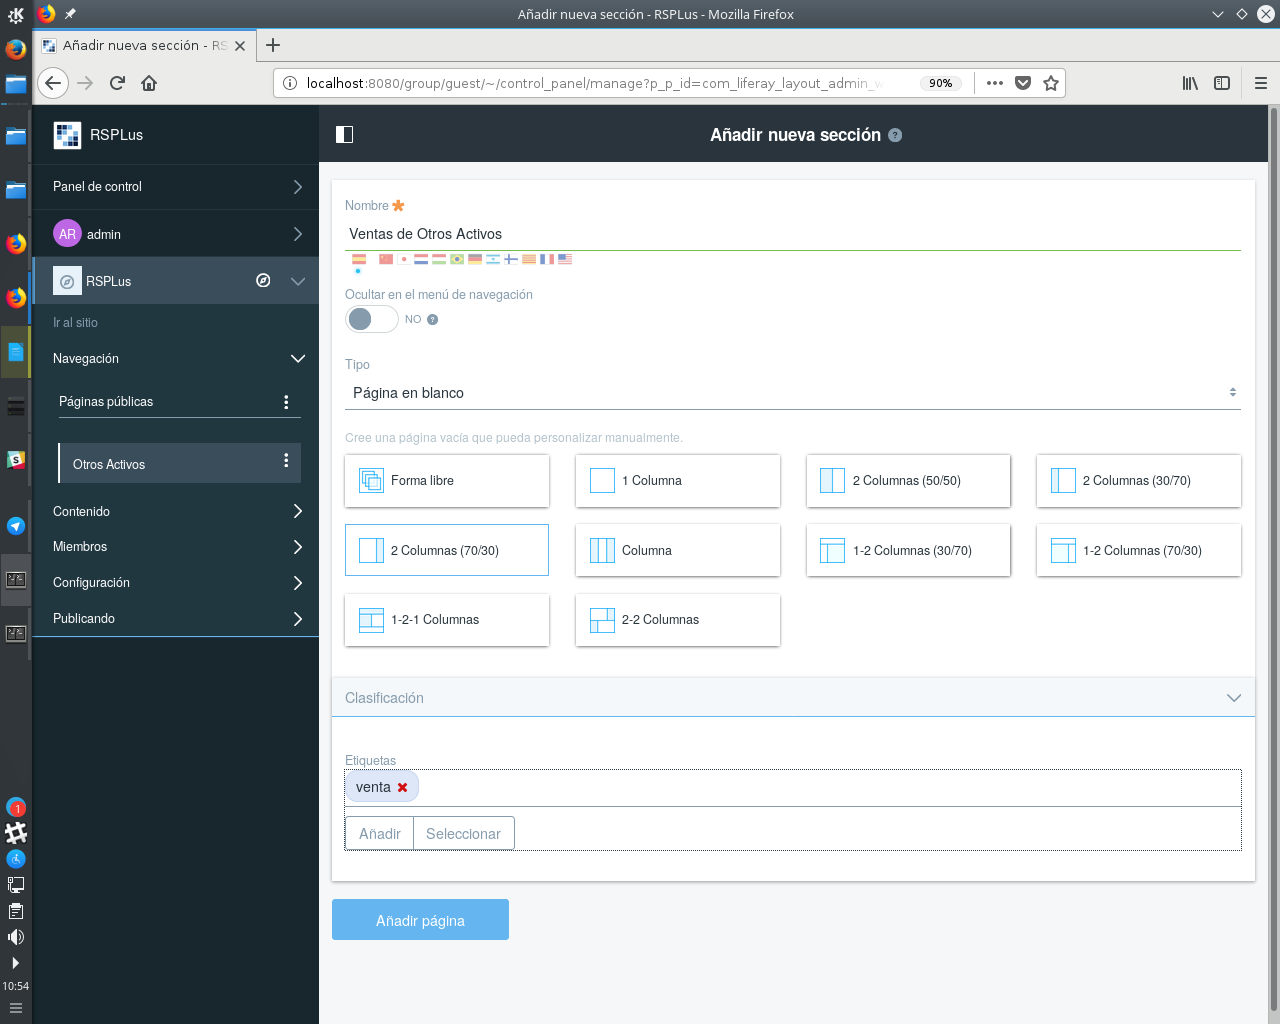
\includegraphics[width=0.8\textwidth]{./img/liferay/5.png}
\end{center}
\caption{Adición de la subpágina de venta}
\label{img:lr5}
\end{figure}

\begin{figure}[H]
\begin{center}
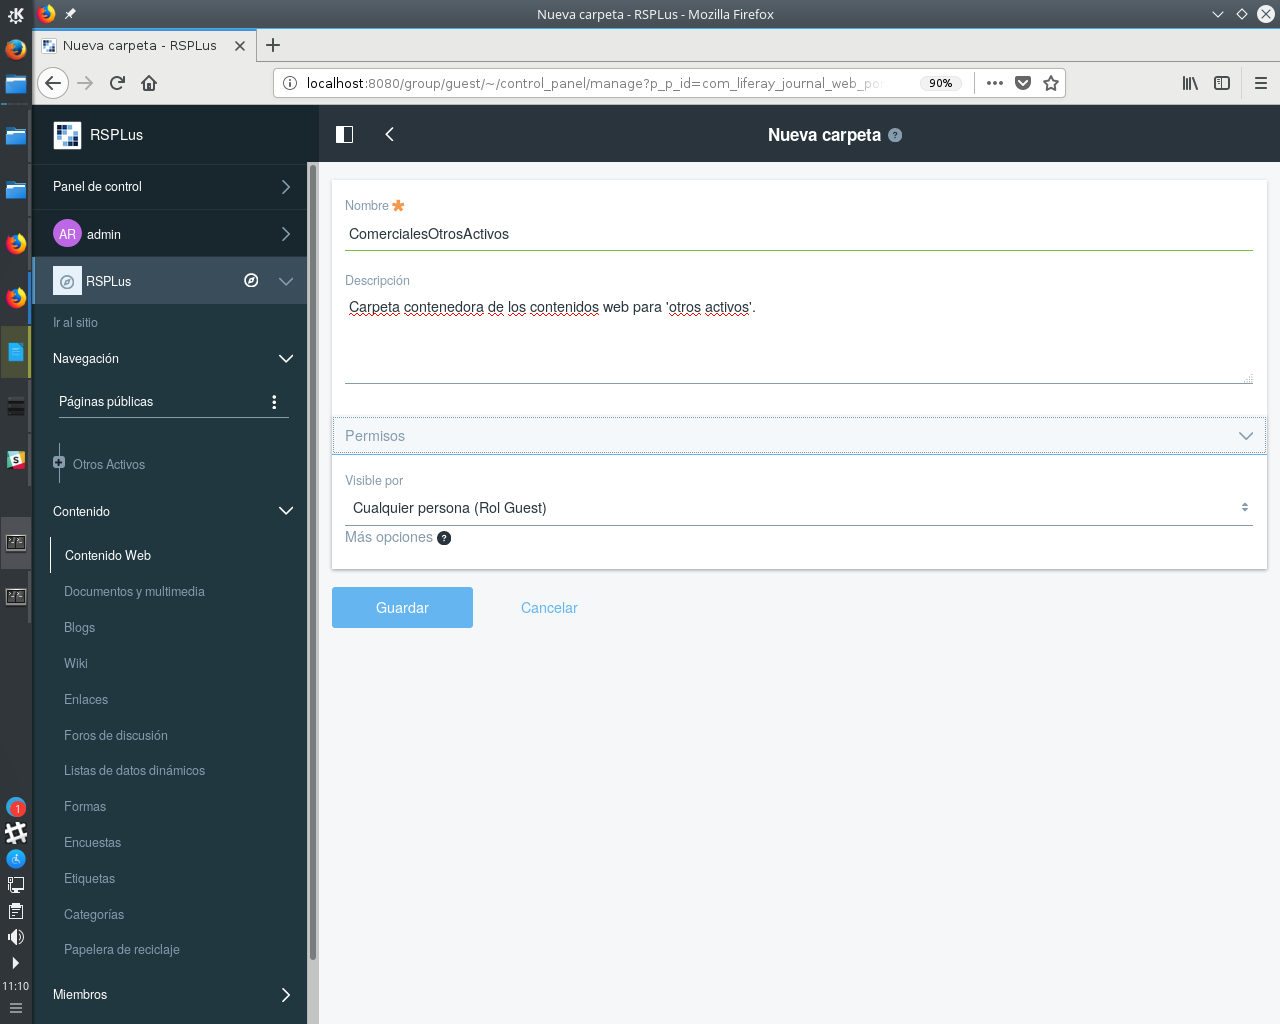
\includegraphics[width=0.8\textwidth]{./img/liferay/6.png}
\end{center}
\caption{Creación de la carpeta Contenidos Web de ComercialesOtrosActivos}
\label{img:lr6}
\end{figure}

\begin{figure}[H]
\begin{center}
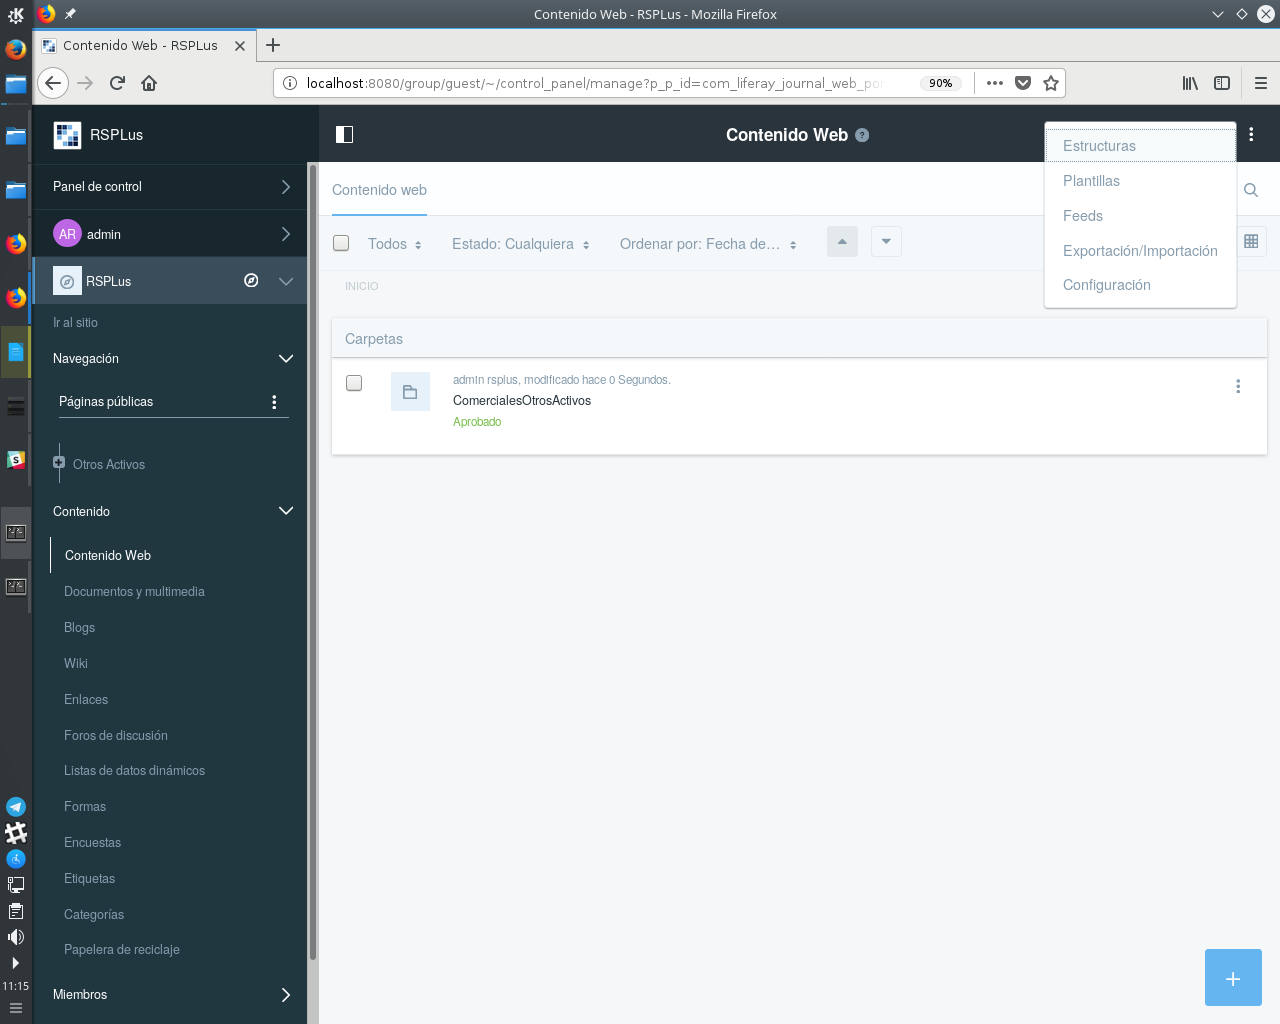
\includegraphics[width=0.8\textwidth]{./img/liferay/7.png}
\end{center}
\caption{Creación de la estructura OtrosActivos}
\label{img:lr7}
\end{figure}

\begin{figure}[H]
\begin{center}
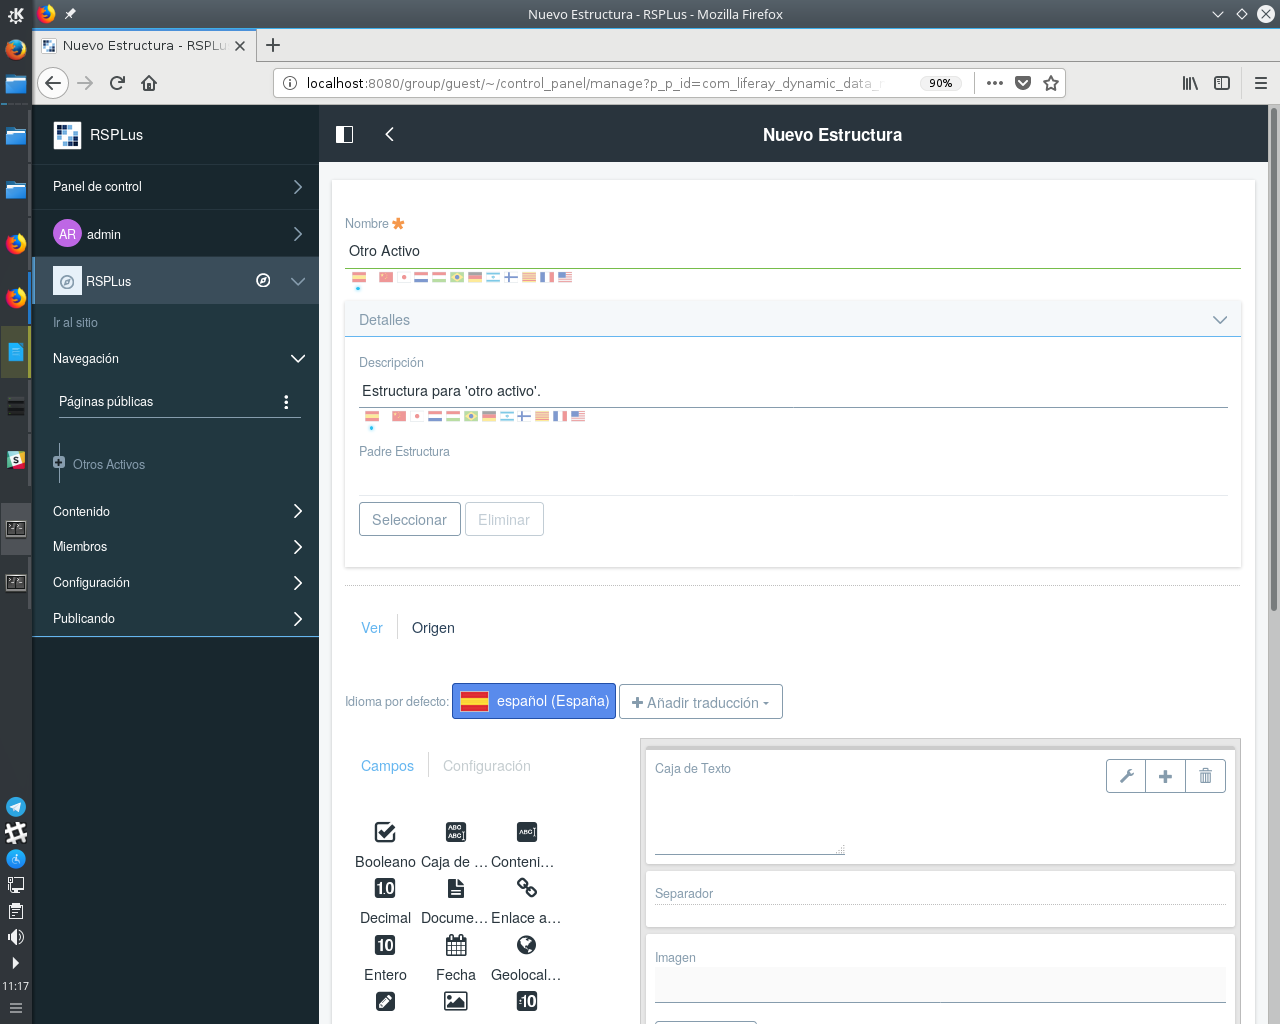
\includegraphics[width=0.8\textwidth]{./img/liferay/8.png}
\end{center}
\caption{Generación de la estructura OtroActivo (paso 1)}
\label{img:lr8}
\end{figure}

\begin{figure}[H]
\begin{center}
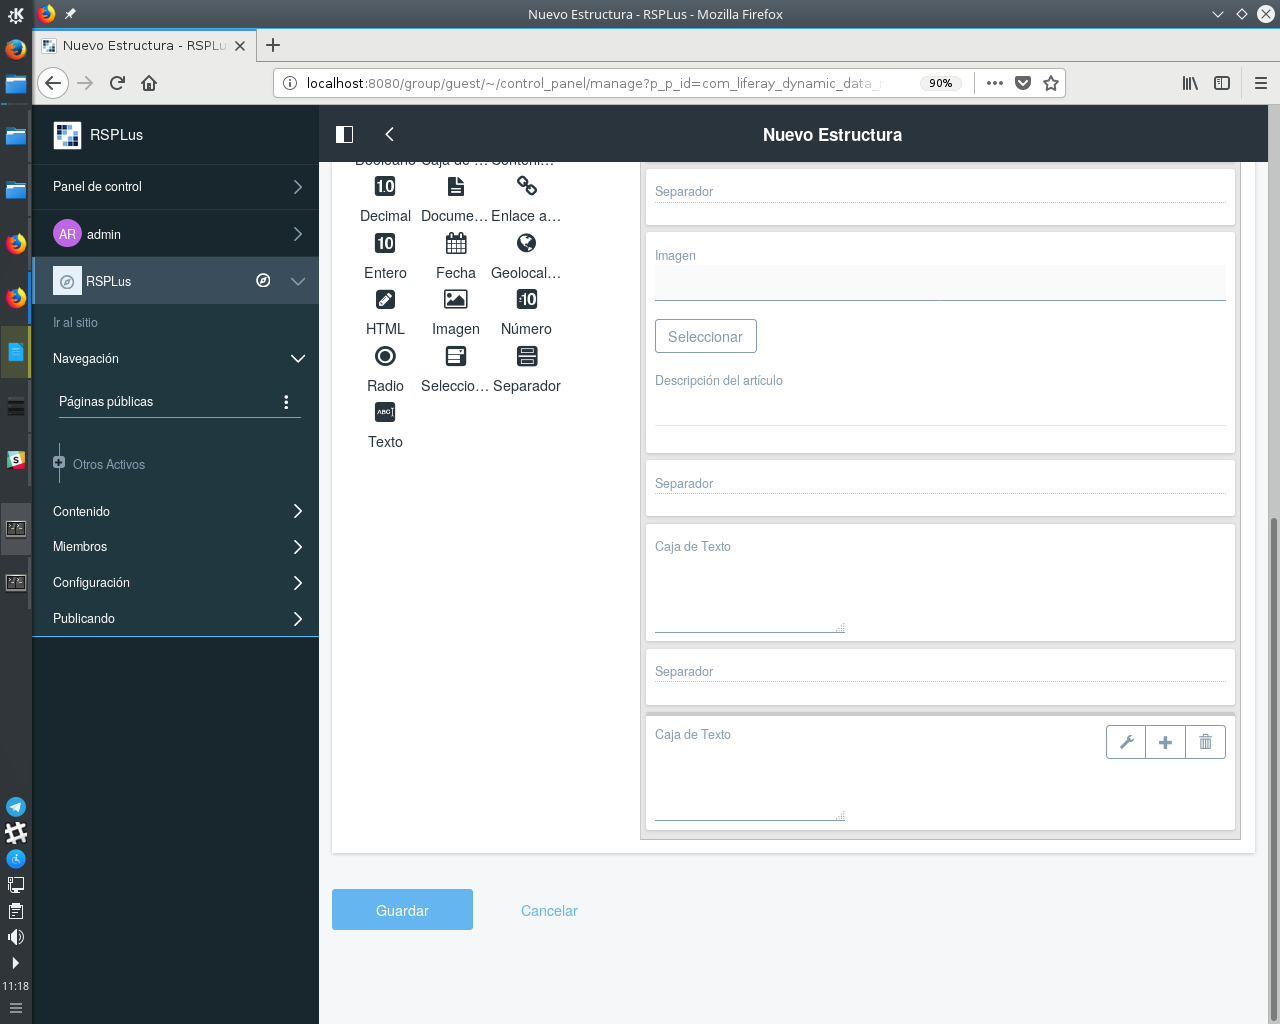
\includegraphics[width=0.8\textwidth]{./img/liferay/9.png}
\end{center}
\caption{Generación de la estructura OtroActivo (paso 2)}
\label{img:lr9}
\end{figure}

\par En la estructura, todos los campos (menos la imagen) deberán ser obligatorios y dependiendo de lo que decida el cliente, se configurarán con unos valores por defecto o no.

\par Una vez creada la estructura, se creará la plantilla \textit{OtroActivo}, como se puede observar en las imágenes \ref{img:lr10} y \ref{img:lr11}.

\begin{figure}[H]
\begin{center}
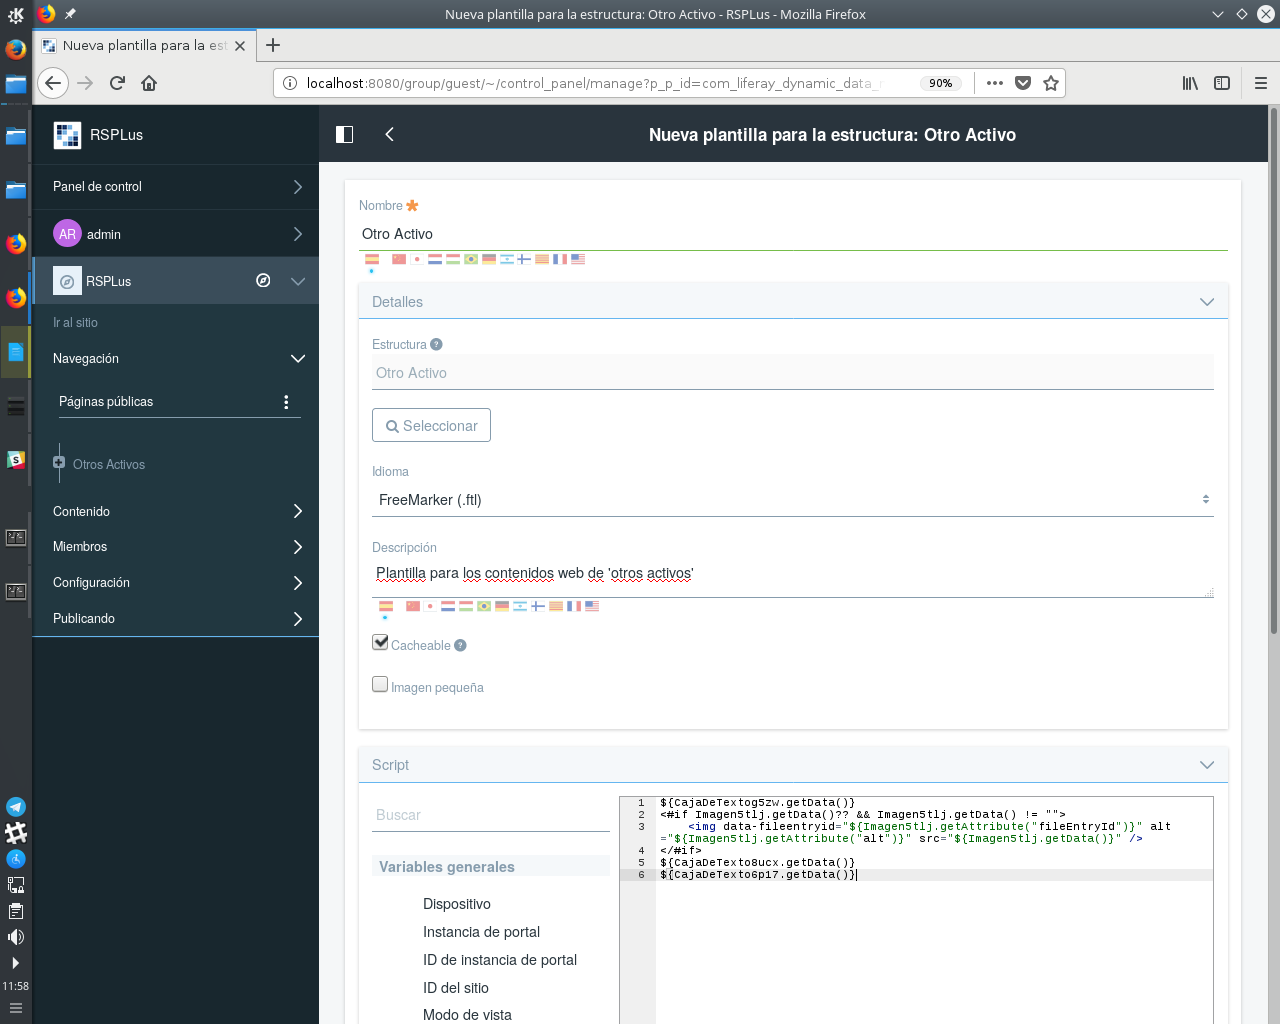
\includegraphics[width=0.8\textwidth]{./img/liferay/10.png}
\end{center}
\caption{Creación de la plantilla OtroActivo (paso 1)}
\label{img:lr10}
\end{figure}

\begin{figure}[H]
\begin{center}
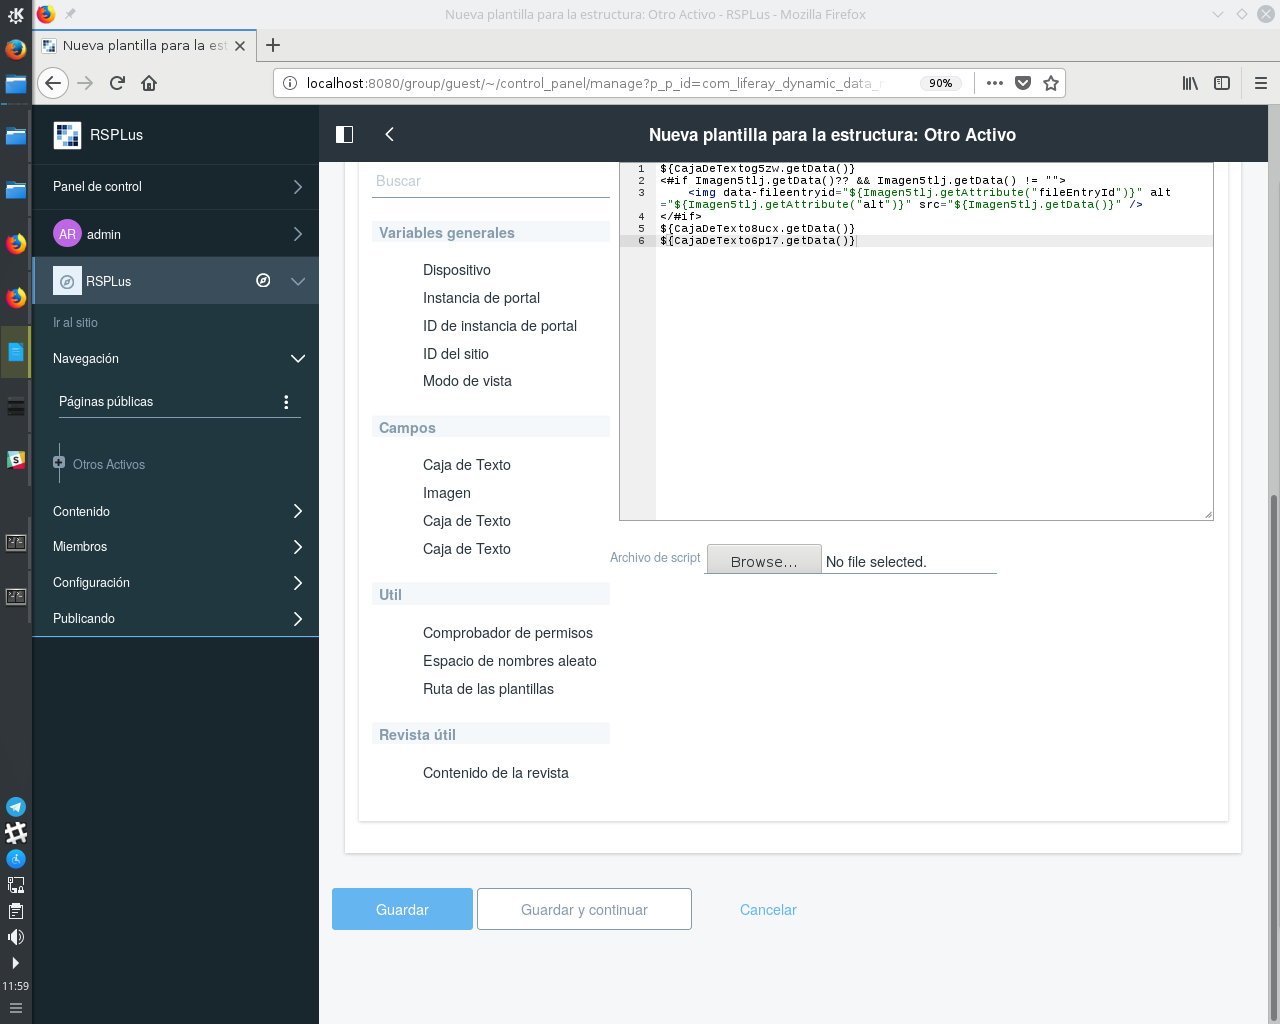
\includegraphics[width=0.8\textwidth]{./img/liferay/11.png}
\end{center}
\caption{Creación de la plantilla OtroActivo (paso 2)}
\label{img:lr11}
\end{figure}

\par Una vez que se dispone de las plantillas y la estructura, se configura la carpeta de contenidos para que sólo se puedan añadir contenidos del tipo 'Otro Activo', así como activar el \textit{workflow de Single Approver} para que los contenidos creados tengan que ser revisados antes de que se publiquen, tal y como se ve en la imagen \ref{img:lr12}.

\begin{figure}[H]
\begin{center}
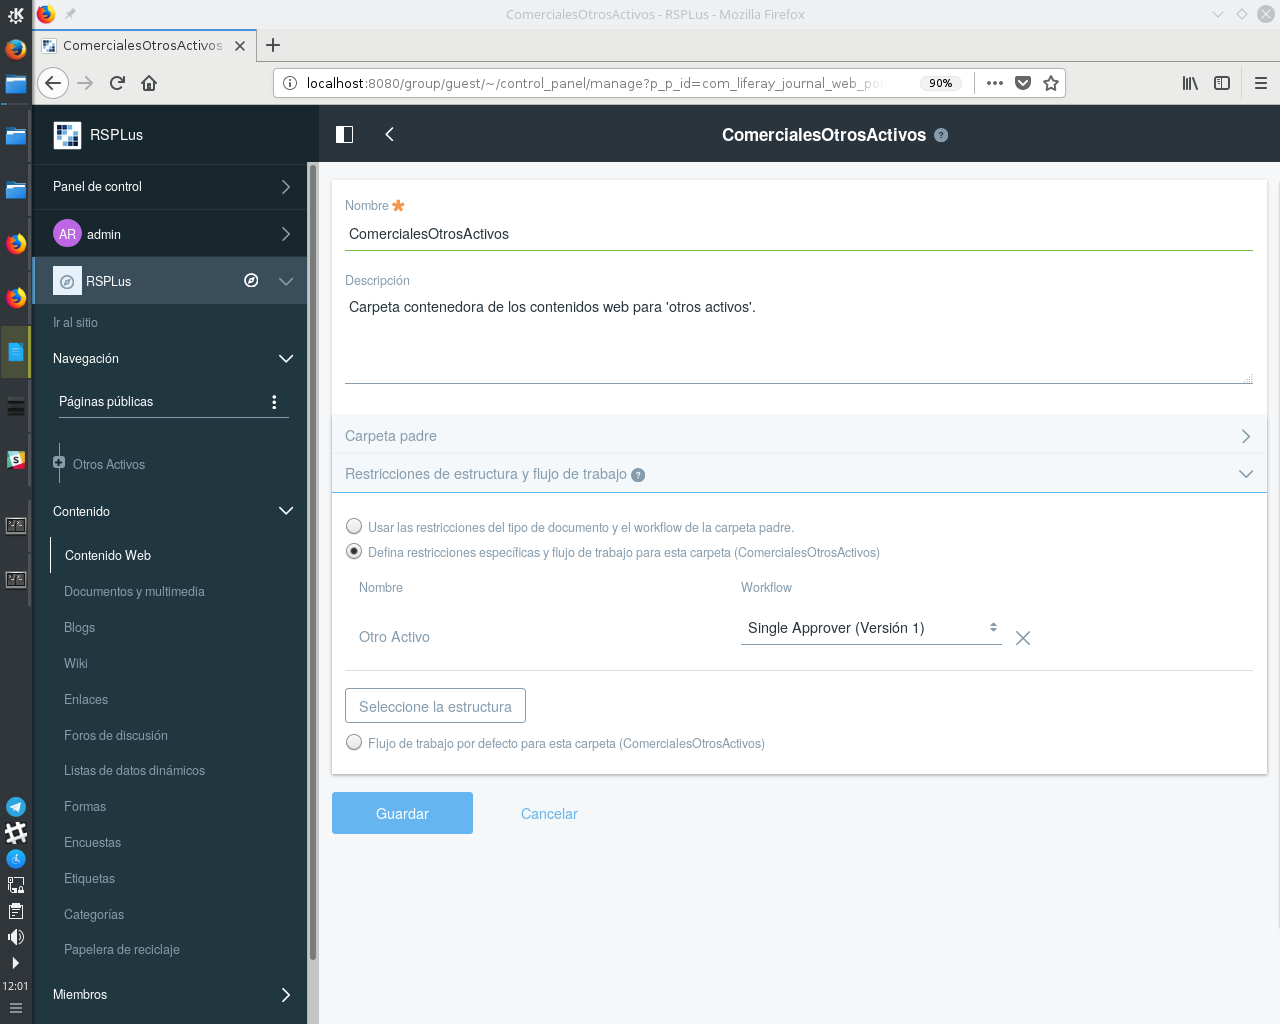
\includegraphics[width=0.8\textwidth]{./img/liferay/12.png}
\end{center}
\caption{Activación del \textit{workflow de Single Approver}}
\label{img:lr12}
\end{figure}

\subsection{Creación de Roles de página}
Desde el panel de control, Usuarios, Rol añadiremos dos roles de sitio web:
\begin{itemize}[-]
    \item Comercial: que tendrá permisos para añadir contenidos a la carpeta que hemos creado antes y contenidos blog, pero nada más.
    \item Publicador: que será prácticamente un administrador de la página, pudiendo añadir páginas, modificarlas, contenidos, blogs y publicar o no los contenidos de la carpeta que hemos creado previamente.
\end{itemize}

\subsubsection{Comercial}
\par Tras la creación del rol de Comercial definida en la figura \ref{img:lr13}, se definen sus permisos, permitiéndole acceder a todo el contenido en relación a los contenidos web, como puede verse en la figura \ref{img:lr14}. De igual manera deben definirse los permisos del mismo para los contenidos del blog (véase figura \ref{img:lr15}).

\begin{figure}[H]
\begin{center}
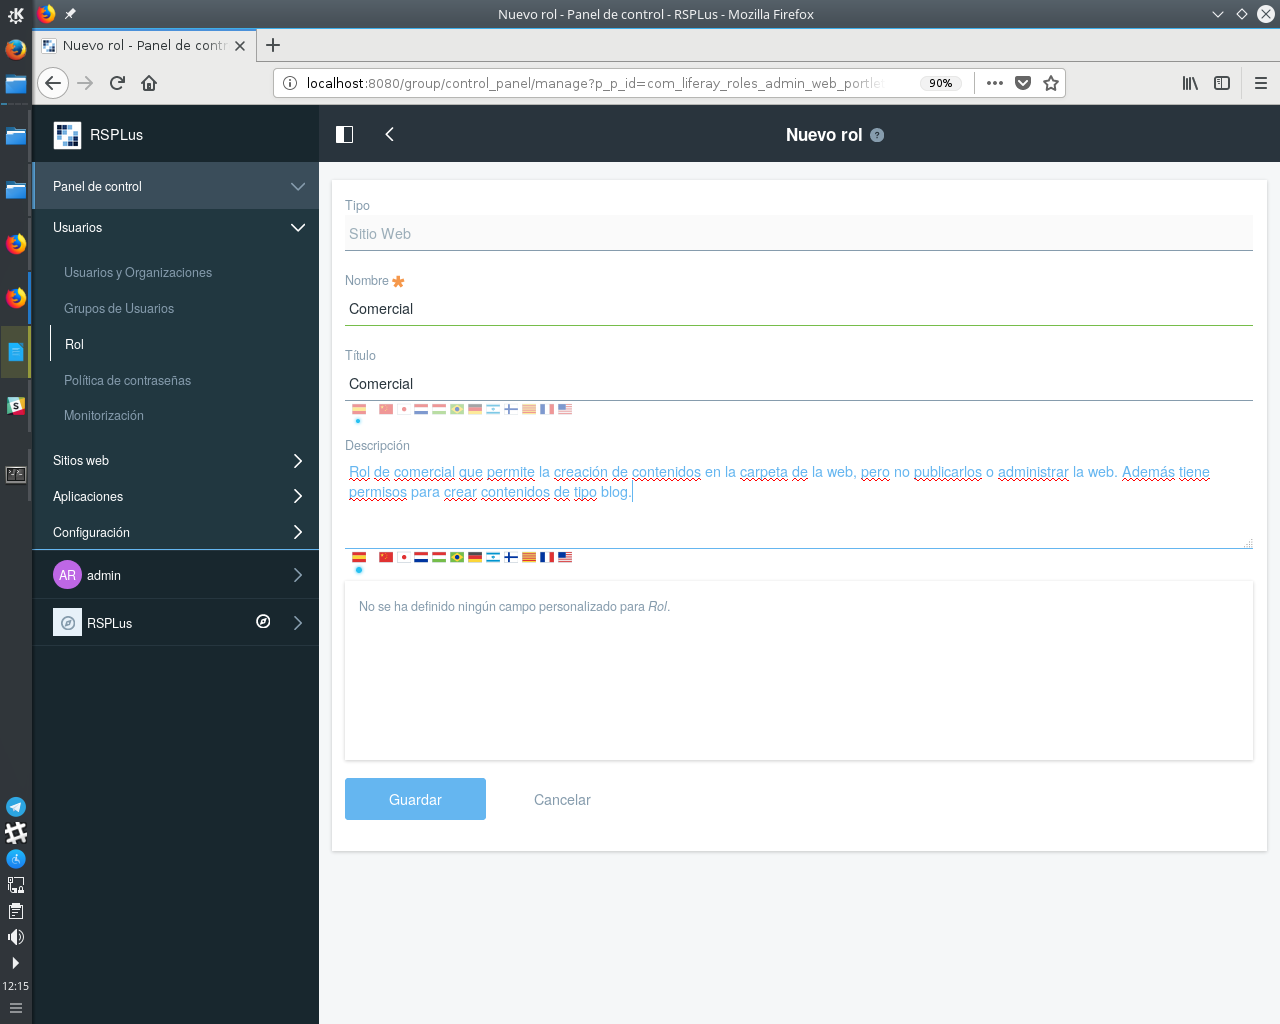
\includegraphics[width=0.8\textwidth]{./img/liferay/13.png}
\end{center}
\caption{Nuevo rol - Comercial}
\label{img:lr13}
\end{figure}

\begin{figure}[H]
\begin{center}
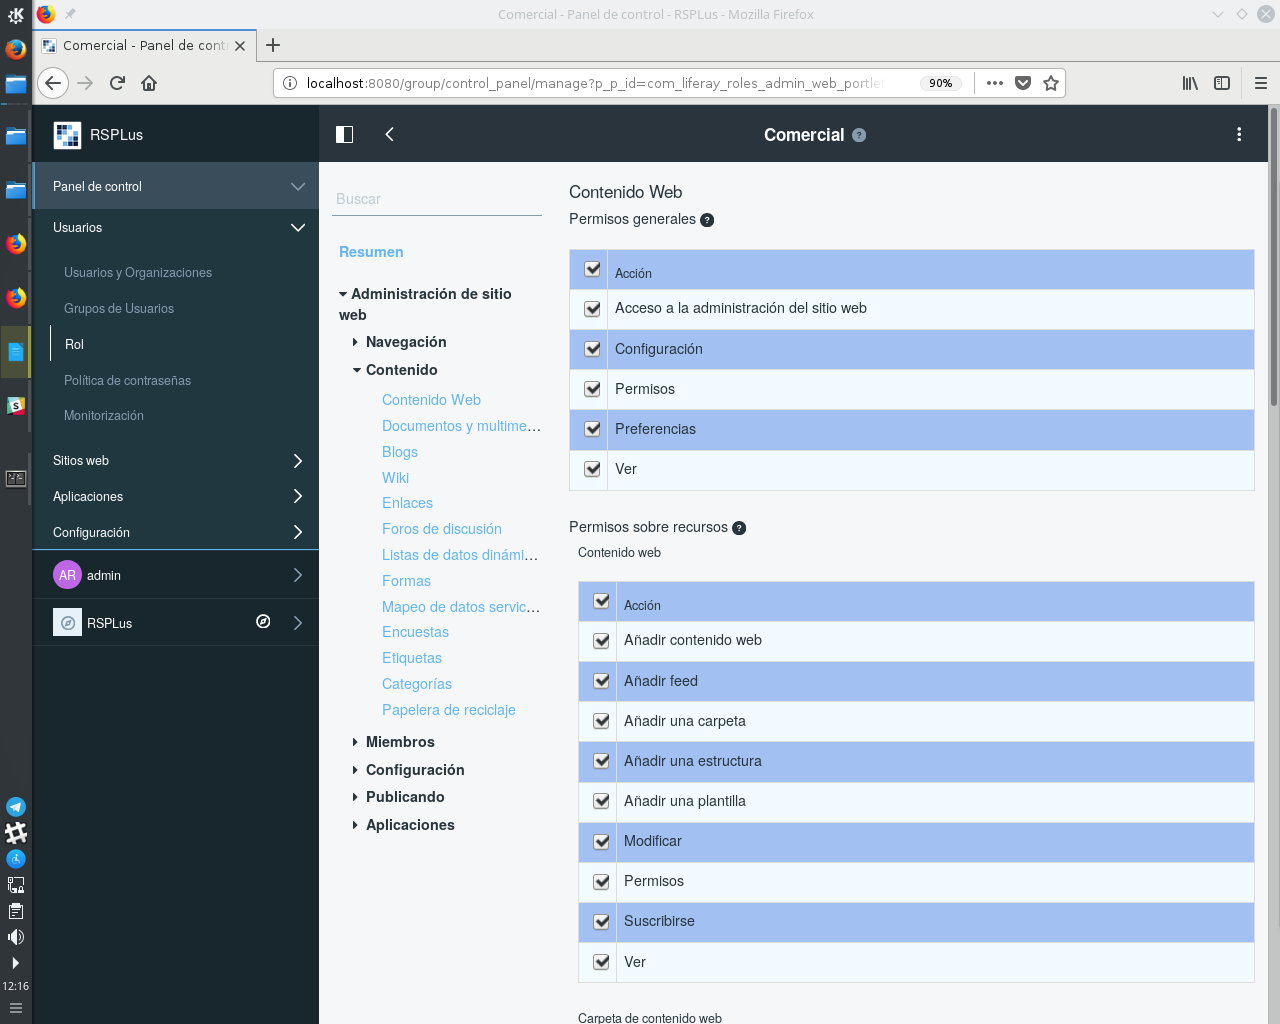
\includegraphics[width=0.8\textwidth]{./img/liferay/14.png}
\end{center}
\caption{Permisos del rol Comercial en el Contenido Web}
\label{img:lr14}
\end{figure}

\begin{figure}[H]
\begin{center}
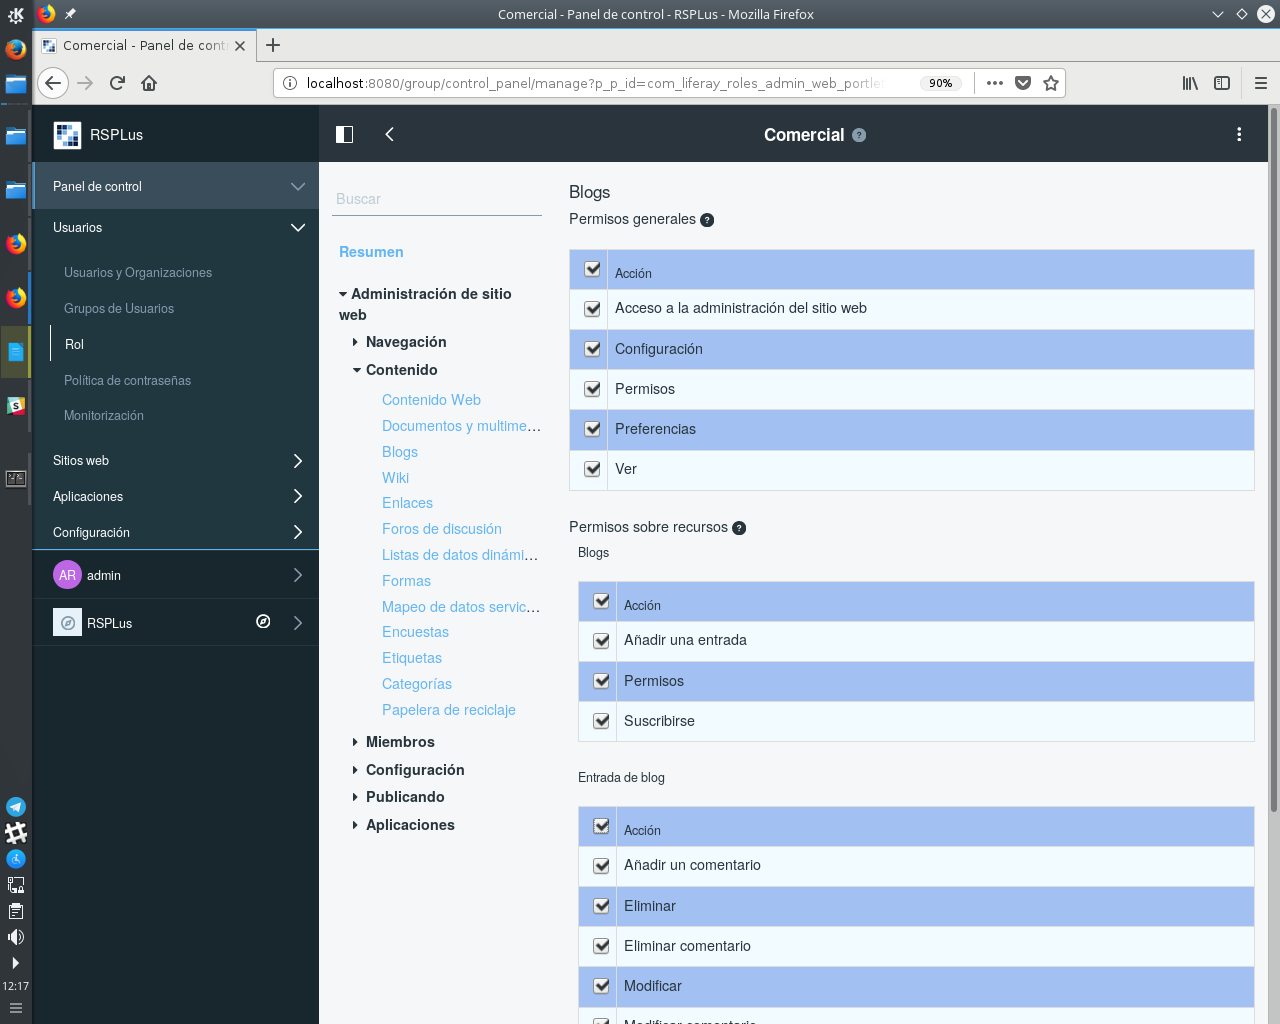
\includegraphics[width=0.8\textwidth]{./img/liferay/15.png}
\end{center}
\caption{Permisos del rol Comercial en el Blog}
\label{img:lr15}
\end{figure}

\subsubsection{Publicador}
\par Tras la creación del rol de Publicador (véase figura \ref{img:lr16}), se deben definir sus permisos tal y como puede observarse en las imágenes \ref{img:lr17}, \ref{img:lr18}, \ref{img:lr19}.

\begin{figure}[H]
\begin{center}
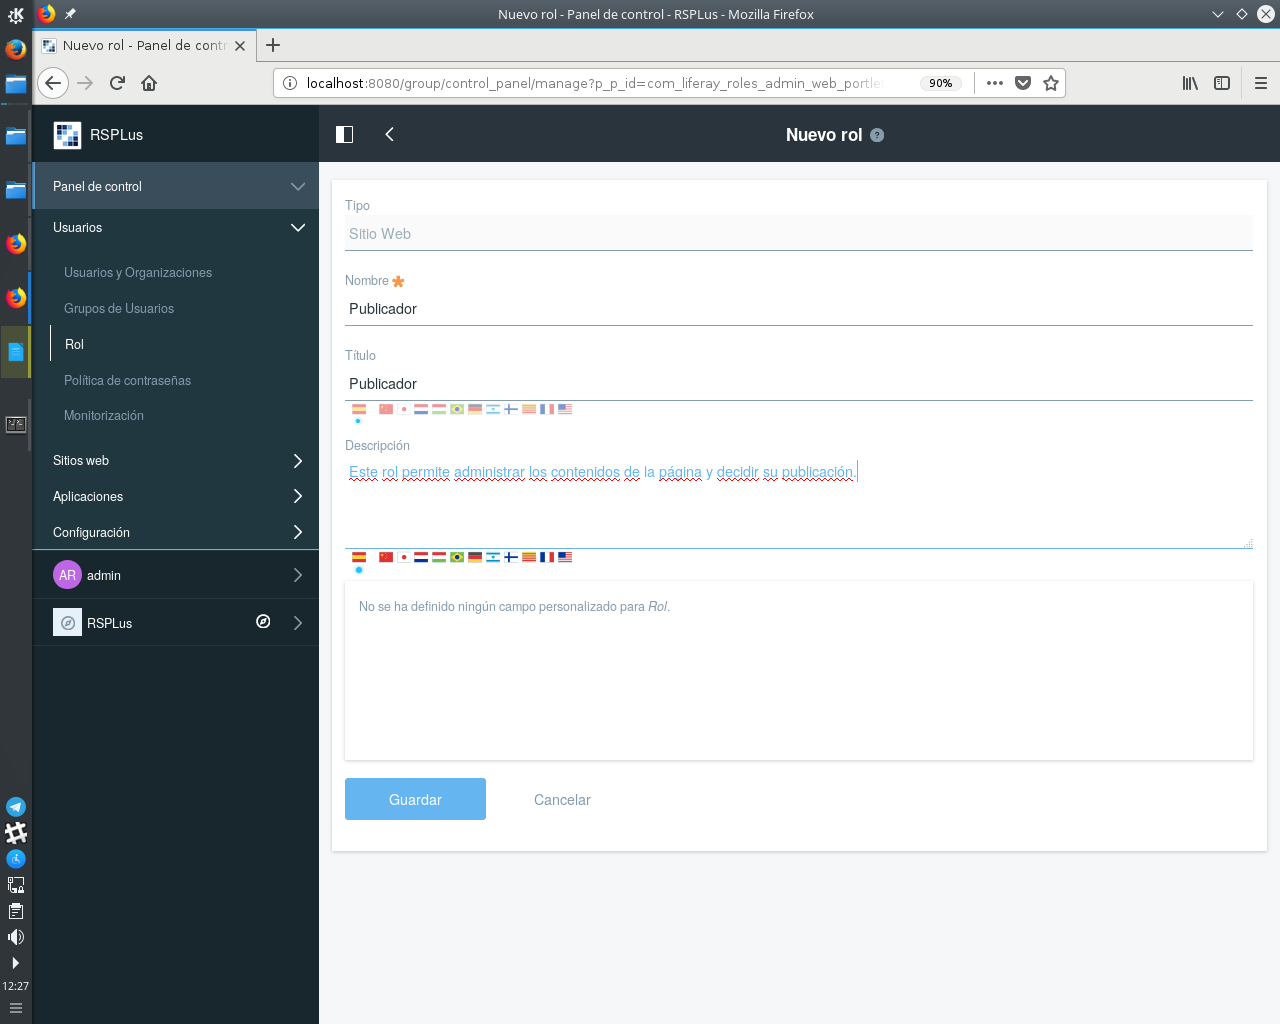
\includegraphics[width=0.8\textwidth]{./img/liferay/16.png}
\end{center}
\caption{Nuevo rol - Publicador}
\label{img:lr16}
\end{figure}

\begin{figure}[H]
\begin{center}
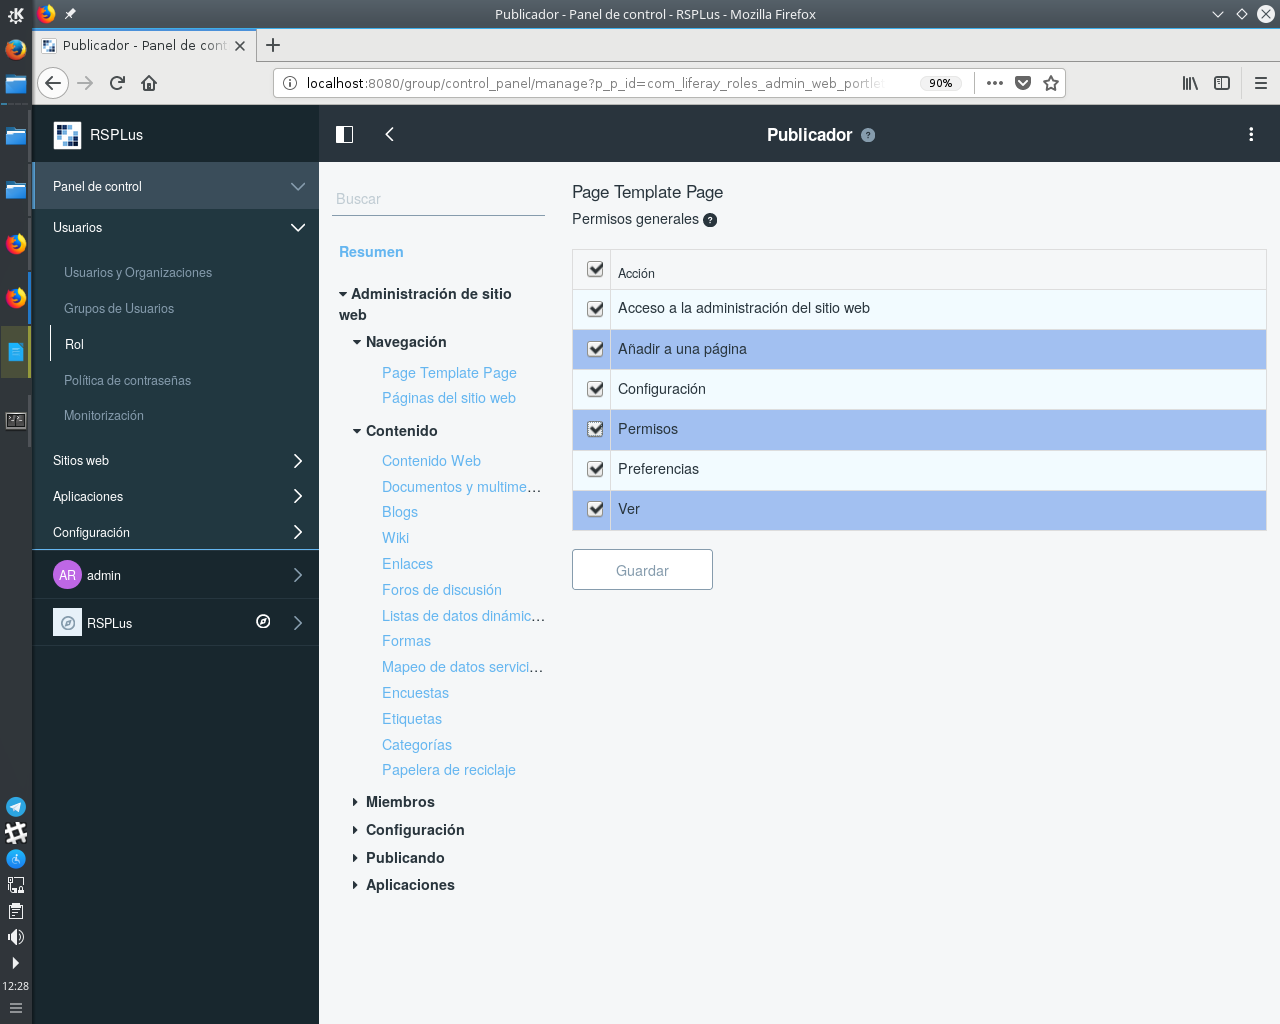
\includegraphics[width=0.8\textwidth]{./img/liferay/17.png}
\end{center}
\caption{Permisos del rol Publicador en el Page Tamplate Page}
\label{img:lr17}
\end{figure}

\begin{figure}[H]
\begin{center}
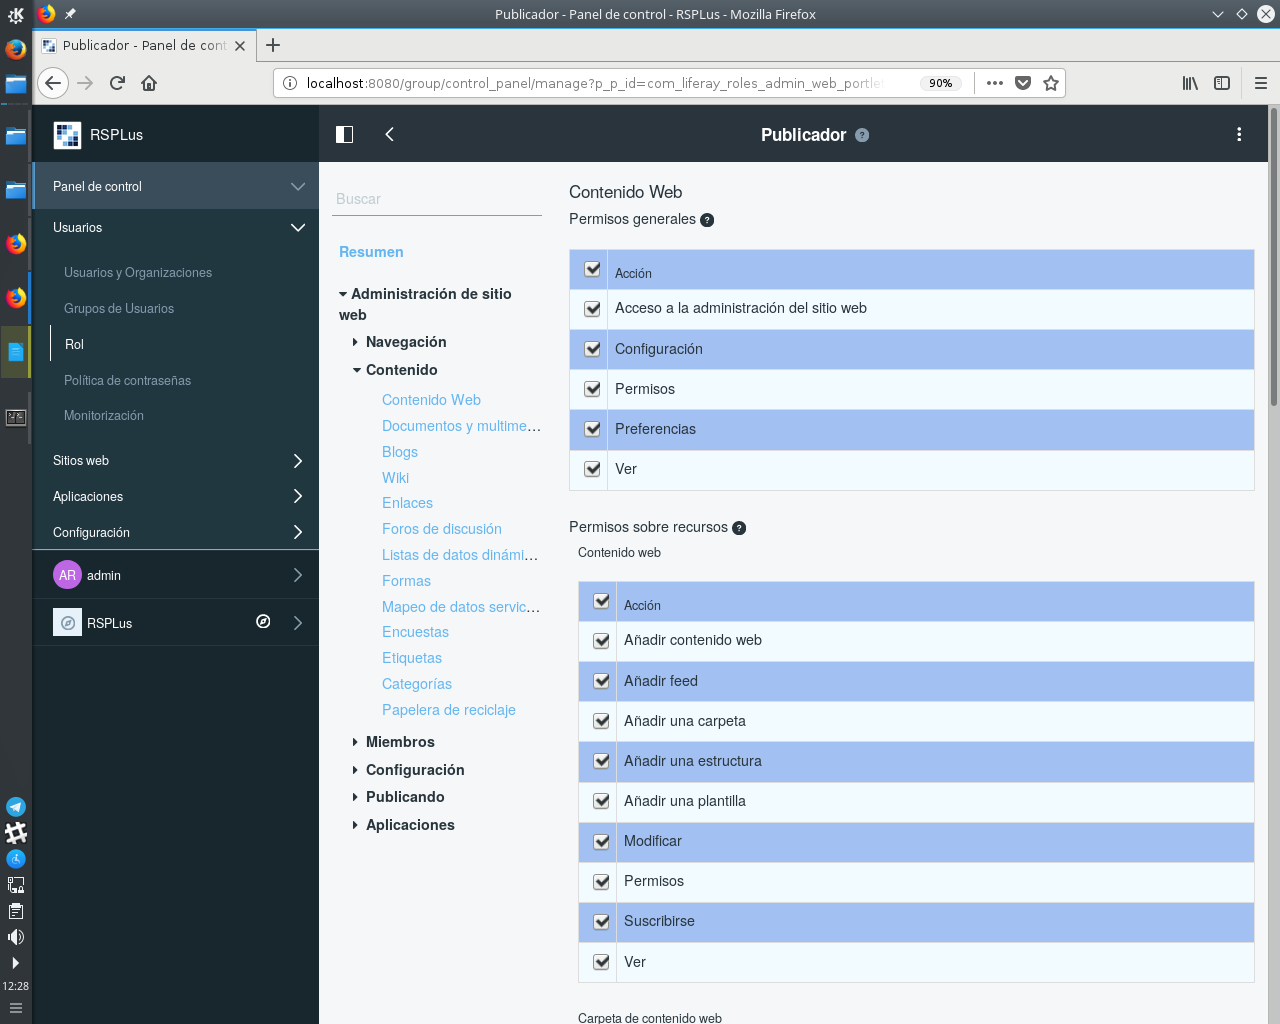
\includegraphics[width=0.8\textwidth]{./img/liferay/18.png}
\end{center}
\caption{Permisos del rol Publicador en el Contenido Web}
\label{img:lr18}
\end{figure}

\begin{figure}[H]
\begin{center}
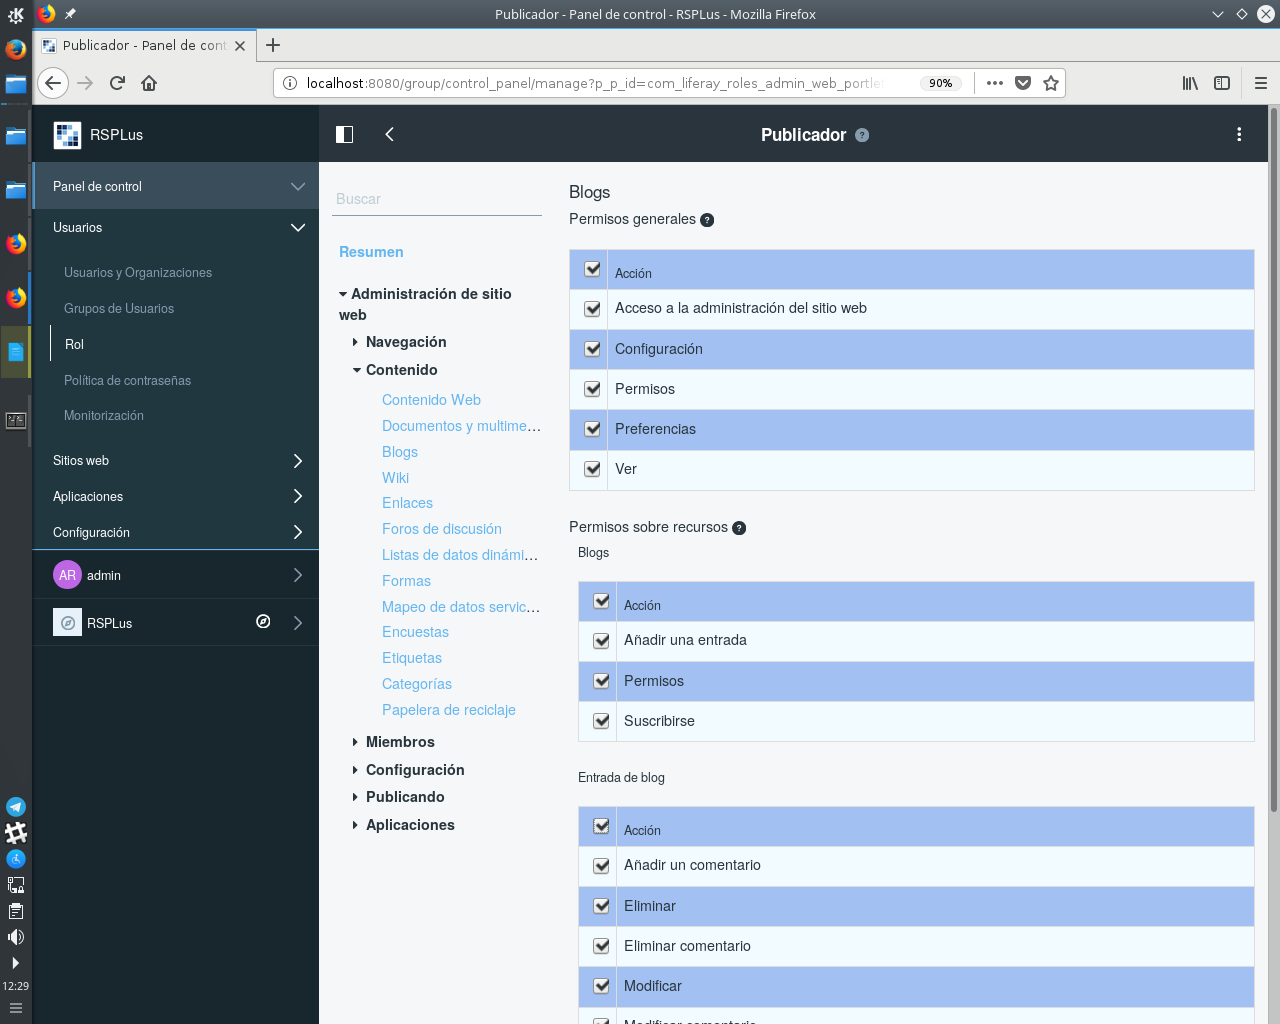
\includegraphics[width=0.8\textwidth]{./img/liferay/19.png}
\end{center}
\caption{Permisos del rol Publicador en el Blog}
\label{img:lr19}
\end{figure}


\subsection{Creación de Usuarios}
\par En esta sección se describirá cómo crear los usuarios que generarán y administrarán el contenido de la página.
\subsubsection{Comercial}
\par Tras agregar \textit{Comercial} a la página (figuras \ref{img:lr20} y \ref{img:lr21}), le debemos asignar sus roles correspondientes (figura \ref{img:lr22}), permitiendo así que el comercial pueda crear contenido web y blogs pero no publicarlo.
\subsubsection{Publicador}
\par Siguiendo los pasos descritos en el apartado anterior y contenidos en las imágenes \ref{img:lr23}, \ref{img:lr24} y \ref{img:lr25} se crea el usuario \textit{Publicador}, permitiéndole publicar la información creada por el Comercial.

\begin{figure}[H]
\begin{center}
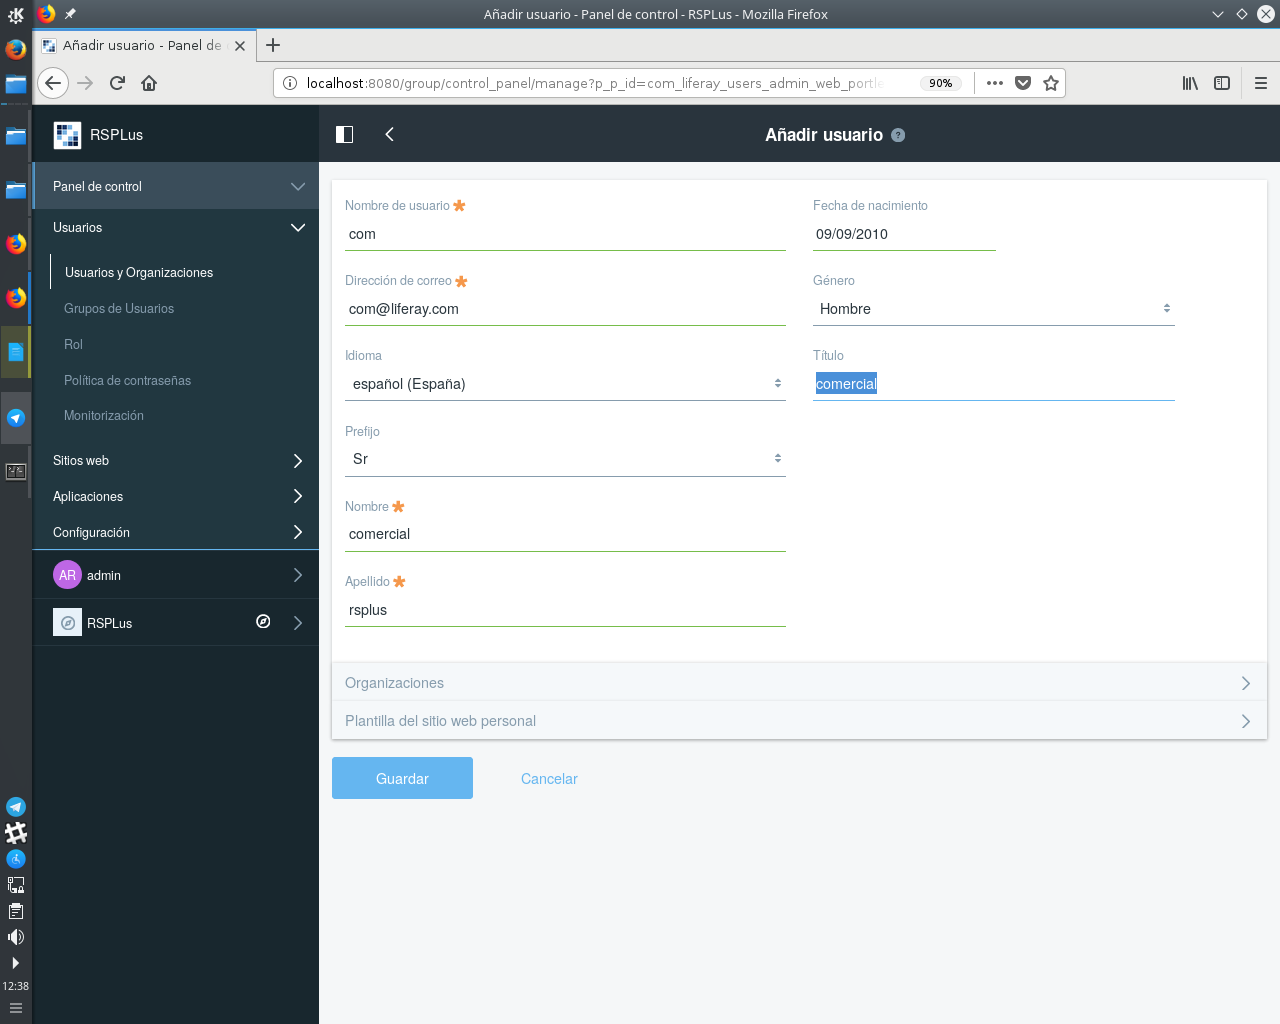
\includegraphics[width=0.8\textwidth]{./img/liferay/20.png}
\end{center}
\caption{Creación de usuario Comercial}
\label{img:lr20}
\end{figure}

\begin{figure}[H]
\begin{center}
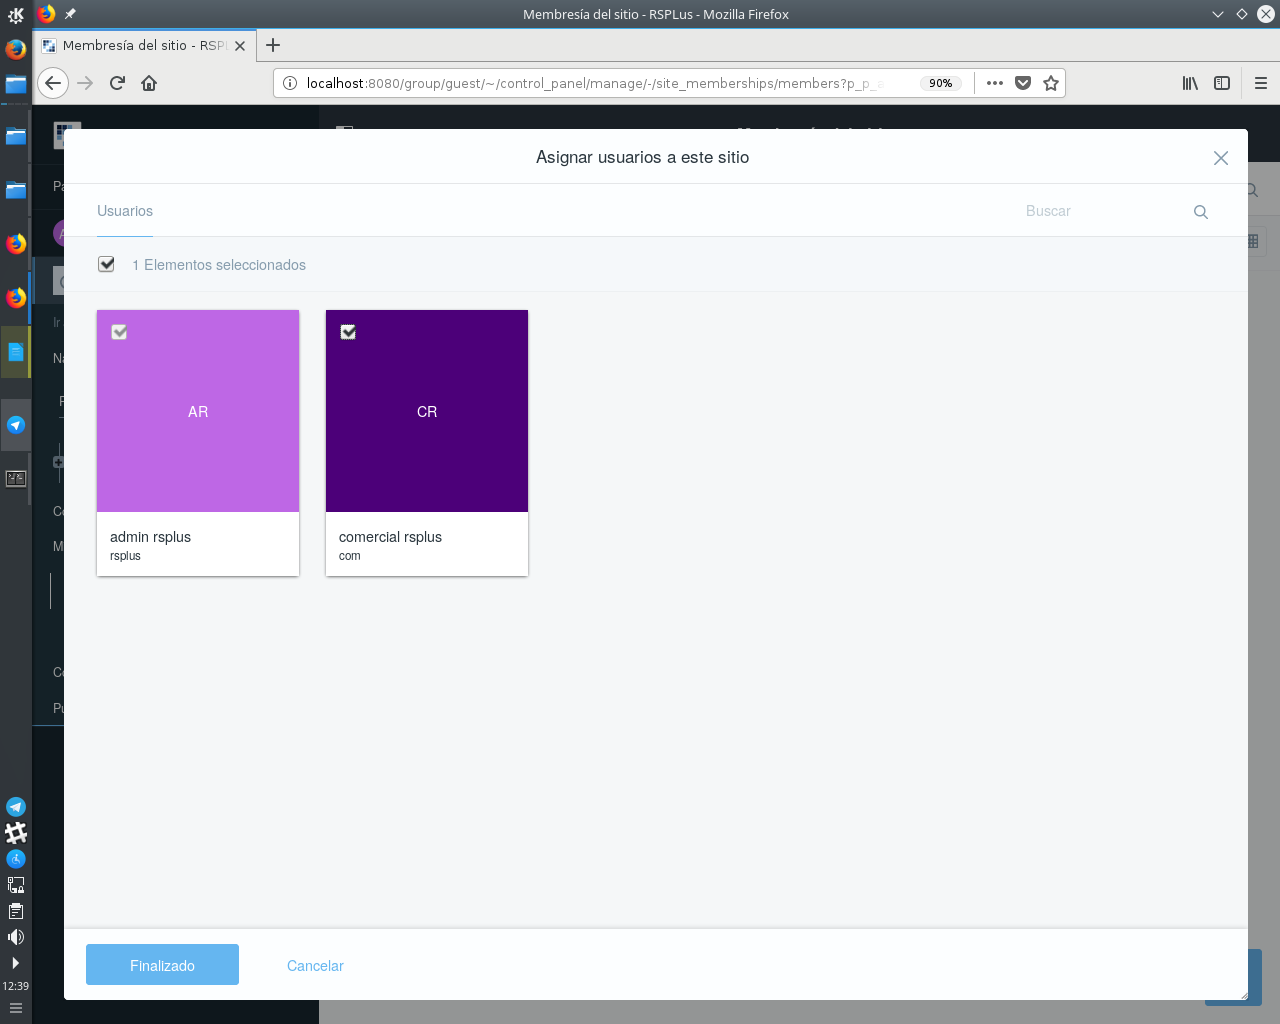
\includegraphics[width=0.8\textwidth]{./img/liferay/21.png}
\end{center}
\caption{Adición del usuario Comercial a la página}
\label{img:lr21}
\end{figure}

\begin{figure}[H]
\begin{center}
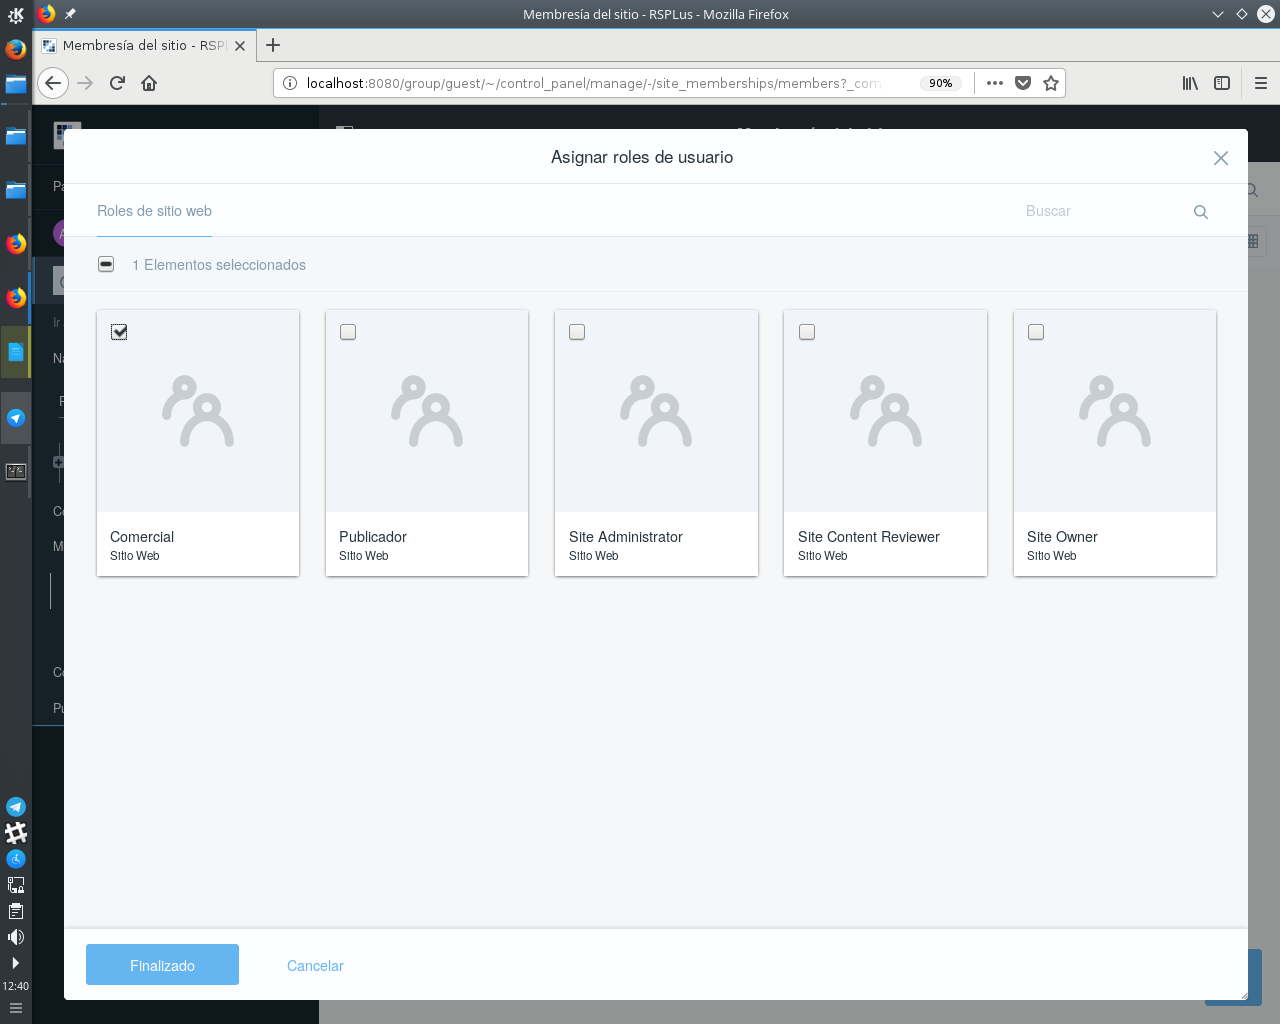
\includegraphics[width=0.8\textwidth]{./img/liferay/22.png}
\end{center}
\caption{Asignación de rol a Comercial}
\label{img:lr22}
\end{figure}

\begin{figure}[H]
\begin{center}
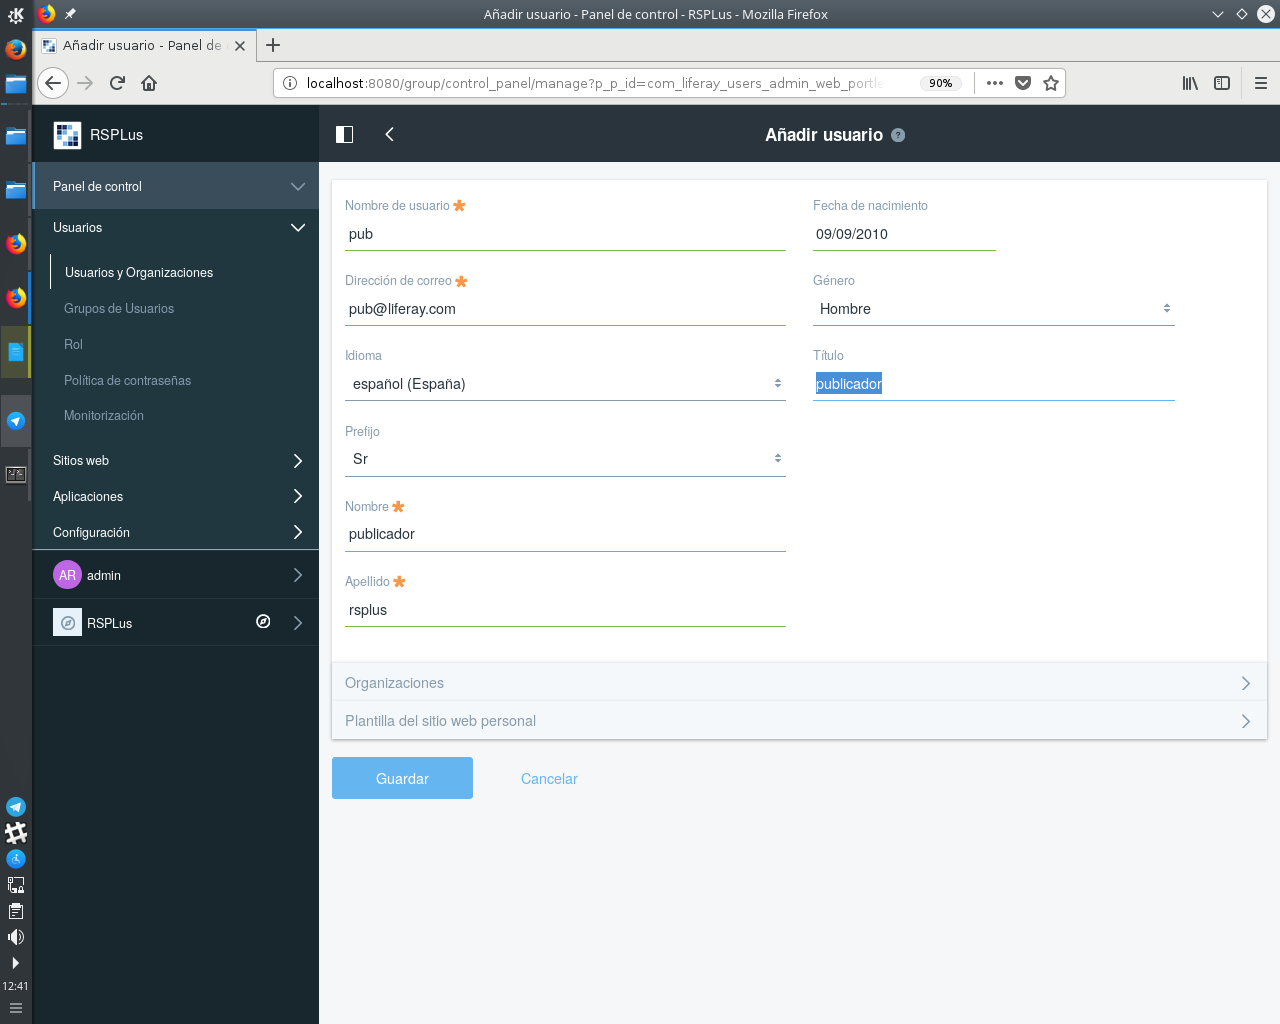
\includegraphics[width=0.8\textwidth]{./img/liferay/23.png}
\end{center}
\caption{Creación de usuario Publicador}
\label{img:lr23}
\end{figure}

\begin{figure}[H]
\begin{center}
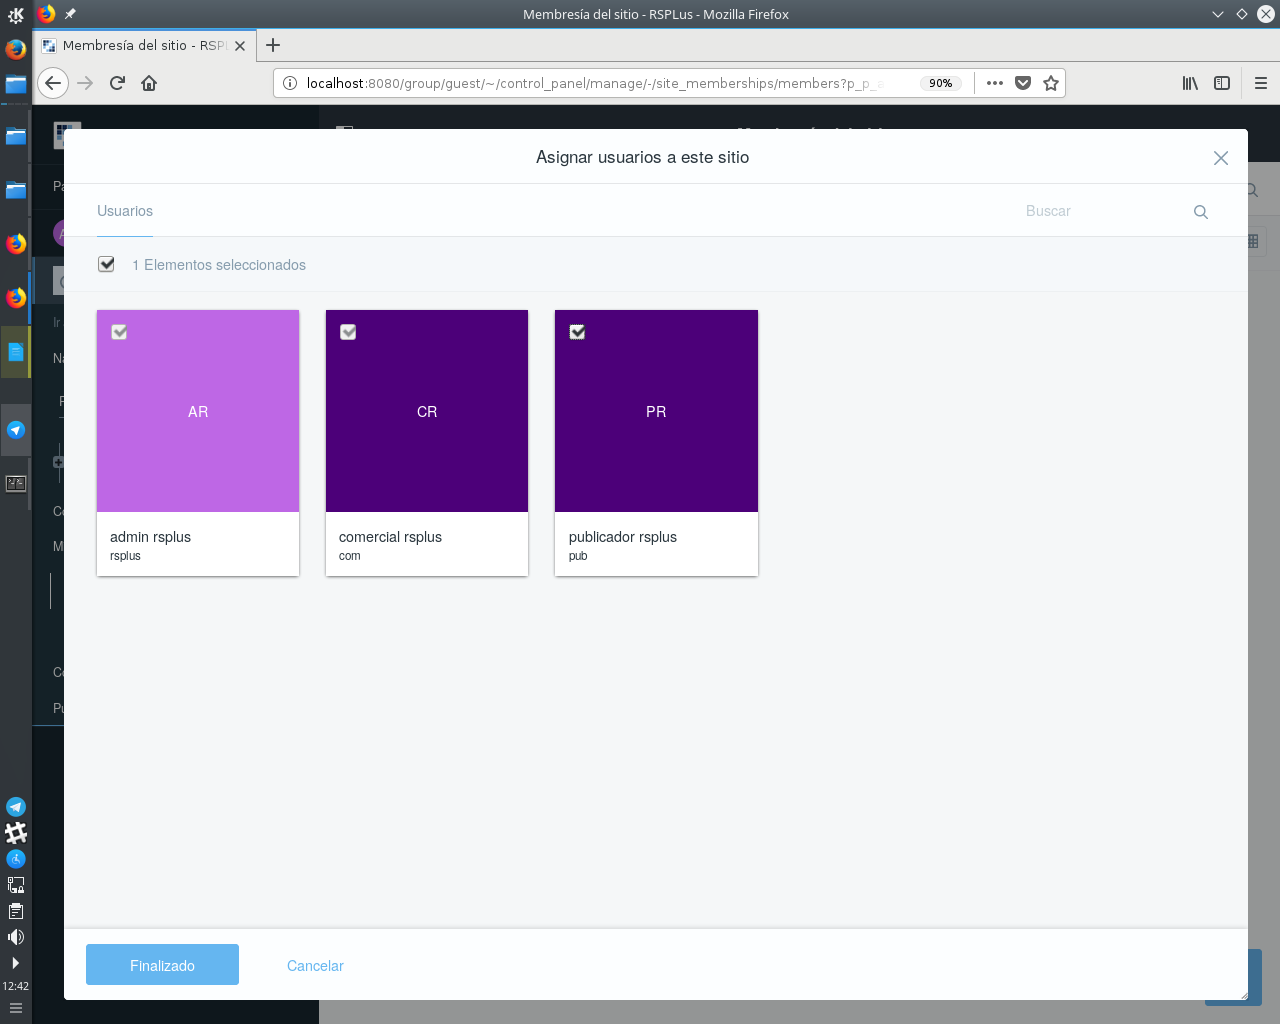
\includegraphics[width=0.8\textwidth]{./img/liferay/24.png}
\end{center}
\caption{Adición del usuario Publicador a la página}
\label{img:lr24}
\end{figure}

\begin{figure}[H]
\begin{center}
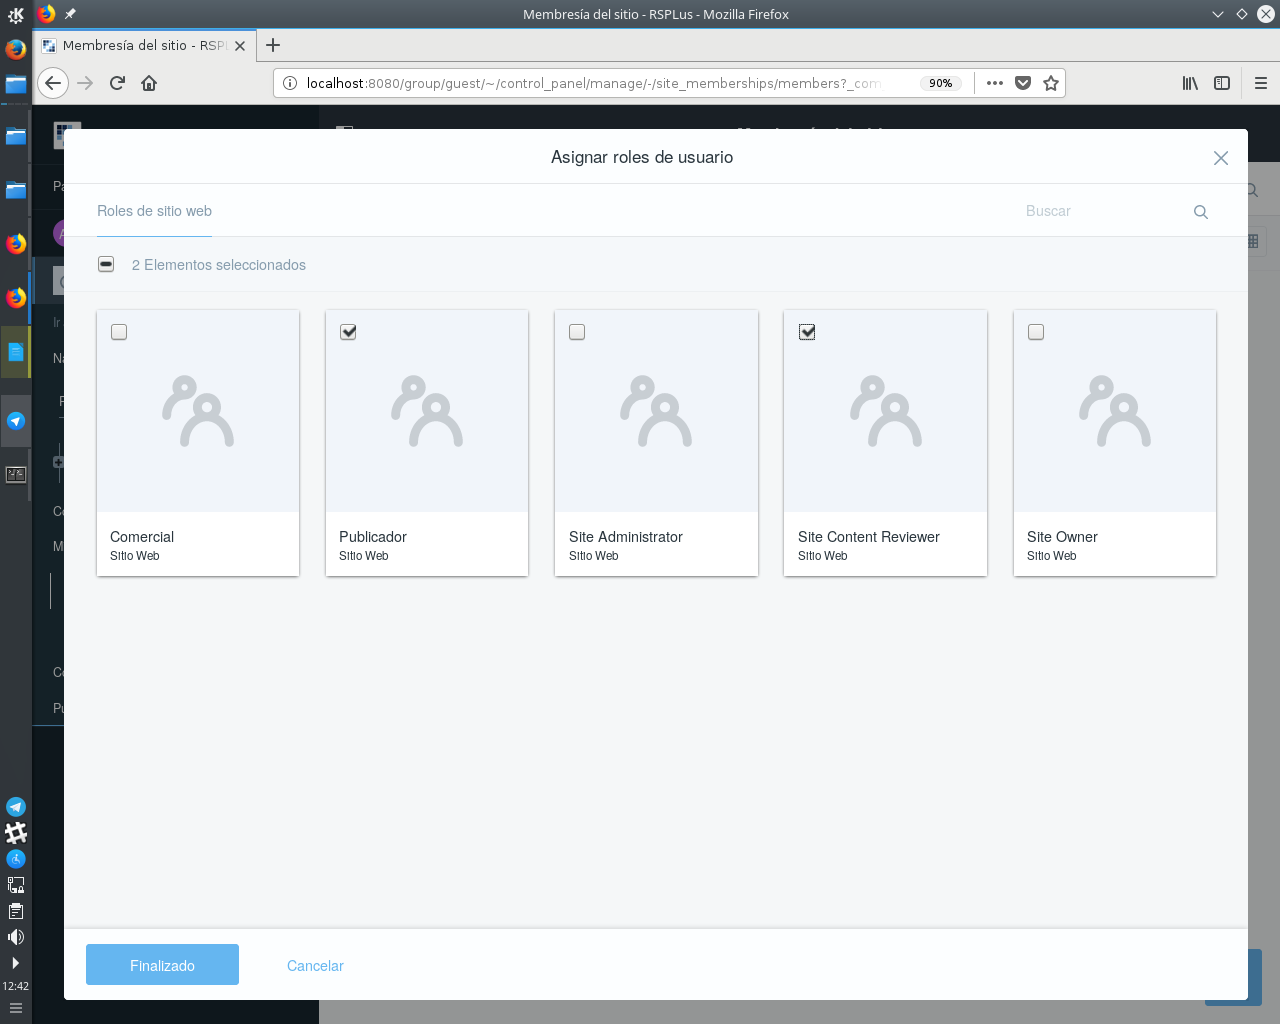
\includegraphics[width=0.8\textwidth]{./img/liferay/25.png}
\end{center}
\caption{Asignación de rol a Publicador}
\label{img:lr25}
\end{figure}

\subsection{Creación del contenido}
A partir de aquí, el cliente puede decidir cómo organizar la página. La recomendación de RSPlus Agency es la siguiente:
\begin{itemize}[-]
    \item En cada subpágina, añadir un Publicador de Contenidos que muestre los contenidos web Otro Activo con el tag que corresponda a la subpágina.
    \item A cada subpágina añadir en la sección de la derecha aplicaciones que muestren al usuario dónde se encuentra como Caminos de Migas, Estructura de la página, etc...
\end{itemize}
